\documentclass[12pt]{report}
\usepackage[utf8]{inputenc}
\usepackage{graphicx}
\usepackage{listings}
\usepackage{color}
\usepackage{hyperref}
\usepackage{geometry}
\usepackage{float}
\usepackage{titlesec}
\usepackage{setspace}
\usepackage{fancyhdr}
\usepackage{array}
\usepackage{enumitem}
\usepackage{tcolorbox}
\usepackage{times}

% Page geometry as per guidelines
\geometry{
    a4paper,
    left=1.5in,
    right=1in,
    top=1in,
    bottom=1in,
    includehead,  % Include space for headers
    includefoot   % Include space for footers
}

% Set line spacing to 1.5
\onehalfspacing

% Format headings as per guidelines
\titleformat{\chapter}[display]
  {\normalfont}
  {\raggedright\fontsize{16}{19}\bfseries\MakeUppercase{\chaptertitlename}\ \thechapter}
  {20pt}
  {\centering\fontsize{18}{22}\bfseries\MakeUppercase}

\titleformat{\section}
  {\normalfont\fontsize{16}{19}\bfseries}{\thesection}{1em}{}

\titleformat{\subsection}
  {\normalfont\fontsize{14}{17}\bfseries}{\thesubsection}{1em}{}

% Set normal text size to 12pt Times New Roman
\renewcommand{\normalsize}{\fontsize{12}{14}\selectfont}

% Remove or comment out the early fancy header setup
% Setup fancy header and footer first
%\pagestyle{fancy}
%\fancyhf{} % Clear all headers and footers
%\fancyhead[L]{Design Thinking Lab Report}
%\fancyhead[R]{Department of ISE}
%\fancyfoot[L]{Academic Year 2024-2025}
%\fancyfoot[R]{\thepage}
%\renewcommand{\headrulewidth}{1pt}
%\renewcommand{\footrulewidth}{1pt}

% Setup chapter page style
%\fancypagestyle{plain}{
%    \fancyhf{} % Clear all headers and footers
%    \fancyhead[L]{Design Thinking Lab Report}
%    \fancyhead[R]{Department of ISE}
%    \fancyfoot[L]{Academic Year 2024-2025}
%    \fancyfoot[R]{\thepage}
%    \renewcommand{\headrulewidth}{1pt}
%    \renewcommand{\footrulewidth}{1pt}
%}

% Title and TOC pages style
\fancypagestyle{empty}{
    \fancyhf{}
    \renewcommand{\headrulewidth}{0pt}
    \renewcommand{\footrulewidth}{0pt}
}

% Ensure chapter pages use fancy style
\renewcommand{\chapterpagestyle}{plain}

% Code styling
\definecolor{codegreen}{rgb}{0,0.6,0}
\definecolor{codegray}{rgb}{0.5,0.5,0.5}
\definecolor{codepurple}{rgb}{0.58,0,0.82}
\definecolor{backcolour}{rgb}{0.95,0.95,0.92}

\lstdefinestyle{mystyle}{
    backgroundcolor=\color{backcolour},   
    commentstyle=\color{codegreen},
    keywordstyle=\color{magenta},
    numberstyle=\tiny\color{codegray},
    stringstyle=\color{codepurple},
    basicstyle=\ttfamily\footnotesize,
    breakatwhitespace=false,         
    breaklines=true,                 
    captionpos=b,                    
    keepspaces=true,                 
    numbers=left,                    
    numbersep=5pt,                  
    showspaces=false,                
    showstringspaces=false,
    showtabs=false,                  
    tabsize=2
}

\lstset{style=mystyle}

% Remove the current chapter style modification
\makeatletter
\renewcommand{\chapter}{\if@openright\cleardoublepage\else\clearpage\fi
    \global\@topnum\z@
    \@afterindentfalse
    \secdef{\@chapter}{\@schapter}}
    
\def\@chapter[#1]#2{\ifnum \c@secnumdepth >\m@ne
    \refstepcounter{chapter}%
    \typeout{\@chapapp\space\thechapter.}%
    \addcontentsline{toc}{chapter}%
        {\protect\numberline{\thechapter}#1}%
    \else
    \addcontentsline{toc}{chapter}{#1}%
    \fi
    \chaptermark{#1}%
    \addtocontents{lof}{\protect\addvspace{10\p@}}%
    \addtocontents{lot}{\protect\addvspace{10\p@}}%
    \@makechapterhead{#2}%
    \@afterheading}
\makeatother

% Title page formatting
\renewcommand{\maketitle}{
    \begin{titlepage}
        \centering
        \vspace*{-2cm}
        
        % Logo and College Name with header
        \begin{center}
            \includegraphics[width=0.9\textwidth]{figures/rvce_logo_header.jpg}\par
        \end{center}
        \vspace{0.5cm}
        
        % Department
        {\Large\bfseries DEPARTMENT OF INFORMATION SCIENCE AND ENGINEERING\par}
        \vspace{0.7cm}
        
        % Lab Report Title
        {\Large\bfseries DESIGN THINKING LAB REPORT\par}
        \vspace{0.3cm}
        {\large IS237DL\par}
        \vspace{0.7cm}

        % Theme and Title
        {\large Theme: IoT in Healthcare\par}
        \vspace{0.3cm}
        {\large Title: HealthHub- A Platform for AI-Driven Health Monitoring and Natural Language Data Querying\par}
        \vspace{1cm}
        
        % Submitted by
        {\large\bfseries Submitted by\par}
        \vspace{0.3cm}
        \begin{tabular}{ll}
            Avinash Anish & USN: 1RV23IS145 \\
        \end{tabular}
        \vspace{1cm}
        
        % Guide
        {\large\bfseries Under the guidance of\par}
        \vspace{0.2cm}
        Dr. Ashwini KB\\
        Associate Professor\\
        Dept. of ISE\\
        RV College of Engineering®\par
        \vfill
        
        % Academic Year
        {\large 2024-2025}
    \end{titlepage}
}

% Add this to control chapter numbering
\setcounter{chapter}{0}

% After the packages and before \begin{document}
% Add these commands for page numbering control
\renewcommand{\thepage}{\roman{page}}  % Roman numerals for preliminary pages

\begin{document}

% Title page with no headers/footers and no page number
\thispagestyle{empty}
\maketitle

% Certificate page
\thispagestyle{empty}
\vspace*{-1.5cm}  % Increased negative space at top
{\centering
\large\bfseries   % Reduced from \Large to \large
RV COLLEGE OF ENGINEERING®,\\
BENGALURU-59\\
\vspace{0.1cm}    % Reduced from 0.2cm
{\small (Autonomous Institution Affiliated to VTU, Belagavi)}\par  % Reduced from normalsize to small
\vspace{0.3cm}    % Reduced from 0.5cm
DEPARTMENT OF INFORMATION SCIENCE AND\\
ENGINEERING\par
\vspace{0.7cm}    % Reduced from 1cm
\includegraphics[width=0.2\textwidth]{figures/rv-logo.png}\par  % Reduced logo size
\vspace{0.7cm}    % Reduced from 1cm
CERTIFICATE\par
}
\vspace{0.3cm}    % Reduced from 0.5cm

\small            % Reduced text size for the main content
\noindent Certified that the Design thinking Laboratory work titled `HealthHub- A Platform for AI-Driven Health Monitoring and Natural Language Data Querying' is carried out by Avinash Anish (1RV23IS145), in partial fulfilment for the requirement of degree of Bachelor of Engineering in Information Science and Engineering of the Visvesvaraya Technological University, Belagavi during the year 2023-2024. It is certified that all corrections/suggestions indicated for the Internal Assessment have been incorporated in the report.

\vspace{0.7cm}    % Reduced from 1cm
\normalsize       % Reset to normal size for signatures
\begin{flushleft}
\hspace{1cm}Dr. Ashwini KB\hfill Dr. Mamatha G.S.\hspace{1cm}\\
\hspace{1cm}Associate Professor\hfill Professor and HoD\hspace{1cm}\\
\hspace{1cm}Department of ISE\hfill Department of ISE\hspace{1cm}
\end{flushleft}

\vspace{1cm}      % Reduced from 1.5cm
\begin{center}
\textbf{External Viva}
\end{center}

\vspace{0.2cm}    % Reduced from 0.3cm
\begin{center}
\begin{tabular}{p{5cm}p{5cm}}
Name of Examiners & Signature with Date\\[0.3cm]
1. & \\[0.2cm]
2. & 
\end{tabular}
\end{center}

\vspace{0.5cm}

\clearpage

% Acknowledgement with Roman numeral page number
\thispagestyle{empty}
{\centering\fontsize{16}{19}\bfseries\spaced{ACKNOWLEDGEMENT}\par}
\vspace{1cm}

\spaced{\noindent Any achievement, be it scholastic or otherwise does not depend solely on the individual efforts but on the guidance, encouragement and cooperation of intellectuals, elders and friends. A number of personalities, in their own capacities have helped us in carrying out this Design Thinking Laboratory work. We would like to take this opportunity to thank them all.}

\vspace{1cm}
\spaced{\noindent We are also thankful to the coordinator, Prof. Sushmitha N, Assistant Professor, Dept. of ISE for her wholehearted support, suggestions and advice during this work.}

\vspace{1cm}
\spaced{\noindent Our sincere thanks to Dr. Mamatha G S, Professor and Head, Department of Information Science and Engineering, RVCE for his support and encouragement.}

\vspace{1cm}
\spaced{\noindent We express sincere gratitude to our beloved Principal, Dr. K. N. Subramanya for his appreciation towards this work.}

\vspace{1cm}
\spaced{\noindent We thank all the teaching staff and technical staff of Information Science and Engineering department, RVCE for their help.}
\clearpage

% Abstract with Roman numeral page number
\thispagestyle{empty}
{\centering\fontsize{16}{19}\bfseries ABSTRACT\par}
\vspace{1cm}

The healthcare information technology market reached USD 260.90 billion in 2023, driven by increasing digitization of health records and rising demand for personalized healthcare solutions. Personal health data management emerged as a critical component in modern healthcare delivery, with Electronic Health Records (EHR) systems and Internet of Things (IoT) devices generating unprecedented volumes of health-related data. Recent developments in Artificial Intelligence (AI) and Machine Learning (ML) have revolutionized how health data is processed, analyzed, and utilized for preventive care and medical decision-making.

Despite these advancements, significant challenges persisted in integrating diverse health data sources and providing contextual, personalized health insights. Traditional health management systems struggled with fragmented data storage, limited interoperability, and inadequate real-time monitoring capabilities. This project addressed these challenges by developing a web-based AI-powered health monitoring platform that seamlessly integrated various data sources while ensuring data privacy and accessibility. The platform aimed to bridge the gap between complex medical information and user comprehension through intelligent data processing and visualization, accessible through any modern web browser.

The development followed the Design Thinking methodology, incorporating five key phases: Empathize, Define, Ideate, Prototype, and Test. The technical implementation utilized the Retrieval-Augmented Generation (RAG) pipeline architecture, built on Next.js 14 for the frontend and FastAPI for the backend services. The system integrated Arduino sensors for real-time health monitoring, employed Large Language Models (LLM) including OpenAI GPT-4o and Google Gemini 2.0 for natural language processing, and utilized Supabase with vector embeddings for efficient data storage and retrieval. The web application was successfully deployed to production using Vercel for the frontend, Amazon Web Services (AWS) for the backend infrastructure, and Supabase Cloud for database services, ensuring high availability and scalability. The project was developed under the assumption of stable internet connectivity and user access to compatible IoT devices, with primary focus on individual health monitoring rather than clinical diagnosis.
\clearpage

% Table of contents with Roman numeral page number
\thispagestyle{empty}
\tableofcontents
\clearpage

% Start headers/footers and Arabic page numbering from here
\pagestyle{fancy}
\fancyhf{} % Clear all headers and footers
\fancyhead[L]{Design Thinking Lab Report}
\fancyhead[R]{Department of ISE}
\fancyfoot[L]{Academic Year 2024-2025}
\fancyfoot[R]{\thepage}
\renewcommand{\headrulewidth}{1pt}
\renewcommand{\footrulewidth}{1pt}

% Setup chapter page style
\fancypagestyle{plain}{
    \fancyhf{} % Clear all headers and footers
    \fancyhead[L]{Design Thinking Lab Report}
    \fancyhead[R]{Department of ISE}
    \fancyfoot[L]{Academic Year 2024-2025}
    \fancyfoot[R]{\thepage}
    \renewcommand{\headrulewidth}{1pt}
    \renewcommand{\footrulewidth}{1pt}
}

% Switch to Arabic numerals and reset page counter
\renewcommand{\thepage}{\arabic{page}}
\setcounter{page}{1}

% Include all sections
\pagestyle{fancy}
\thispagestyle{fancy}
\chapter{Empathy}
\section{Introduction to Empathy}
Our design process began with a deep dive into understanding the challenges faced by individuals in managing their personal health information. Through extensive user research, we identified several key pain points:

\begin{itemize}
    \item Fragmentation of health records across multiple platforms and providers
    \item Difficulty in interpreting medical data and test results
    \item Challenge of tracking real-time health metrics
    \item Need for personalized health insights
\end{itemize}

\section{Customer Persona and Environment}
Based on our research, we developed primary user personas representing our target users:

\begin{itemize}
    \item Health-conscious individuals managing chronic conditions
    \item Active adults tracking fitness and nutrition goals
    \item Caregivers managing health information for family members
    \item Healthcare providers seeking efficient patient data access
\end{itemize}

\section{Customer Journey Map}
\begin{figure}[H]
    \centering
    \includegraphics[width=1.0\textwidth]{figures/customer_journey_map.png}
    \caption{Figure 1.1: Customer Journey Map}
\end{figure}

Key journey stages identified:
\begin{enumerate}
    \item Initial Health Data Collection
    \item Record Organization and Storage
    \item Data Analysis and Interpretation
    \item Health Insight Generation
    \item Action Planning and Implementation
\end{enumerate}

\section{Customer Empathy Maps}

\begin{figure}[H]
    \centering
    \includegraphics[width=0.8\textwidth]{figures/patient_empathy_map.png}
    \caption{Figure 1.2: Patient Empathy Map Visualization}
\end{figure}

\begin{figure}[H]
    \centering
    \includegraphics[width=0.8\textwidth]{figures/developer_empathy_map.png}
    \caption{Figure 1.3: Healthcare Developer Empathy Map Visualization}
\end{figure}

\subsection{Says}
\begin{itemize}
    \item "I need all my medical documents in one place"
    \item "Which portal has my latest scan results?"
    \item "I wish I could just search through all my reports at once"
\end{itemize}

\subsection{Thinks}
\begin{itemize}
    \item Managing all these documents is overwhelming
    \item What if I miss something important?
    \item There must be a better way to organize all this
\end{itemize}

\subsection{Does}
\begin{itemize}
    \item Takes photos of every medical document
    \item Maintains multiple folders for different tests
    \item Manually enters test results in spreadsheets
\end{itemize}

\subsection{Feels}
\begin{itemize}
    \item Frustrated when can't find specific test results
    \item Anxious about keeping track of everything
    \item Overwhelmed by different portals and systems
\end{itemize}

\section{Tools used for Empathy}
\subsection{Customer Survey and Analysis}
We conducted a comprehensive survey with 120 respondents to understand user needs and behaviors regarding health monitoring and data management.

\begin{minipage}{0.5\textwidth}
\textbf{Demographics}\\
Our survey reached a diverse group of participants:
\begin{itemize}
    \item 101 respondents aged 18-25
    \item 103 students
    \item 12 caregivers/family members
\end{itemize}
\end{minipage}
\begin{minipage}{0.5\textwidth}
\begin{figure}[H]
    \centering
    \includegraphics[width=0.9\textwidth]{figures/demographics_pie.png}
    \caption{Figure 1.4: Distribution of Survey Respondents by Role}
\end{figure}
\end{minipage}

\begin{minipage}{0.5\textwidth}
\textbf{Health Monitoring Habits}\\
The frequency of health monitoring varied among respondents:
\begin{itemize}
    \item 59 people - Only during doctor visits
    \item 25 people - Weekly monitoring
    \item 19 people - Monthly monitoring
\end{itemize}
\end{minipage}
\begin{minipage}{0.5\textwidth}
\begin{figure}[H]
    \centering
    \includegraphics[width=0.9\textwidth]{figures/monitoring_frequency.png}
    \caption{Figure 1.5: Health Monitoring Frequency Distribution}
\end{figure}
\end{minipage}

\begin{minipage}{0.5\textwidth}
\textbf{Health Records Management}\\
Current methods of health record storage:
\begin{itemize}
    \item 45\% use paper records
    \item 32\% use health apps (Apple Health, MyChart)
    \item 23\% use other methods
\end{itemize}
\end{minipage}
\begin{minipage}{0.5\textwidth}
\begin{figure}[H]
    \centering
    \includegraphics[width=0.9\textwidth]{figures/records_storage.png}
    \caption{Figure 1.6: Health Records Storage Methods}
\end{figure}
\end{minipage}

\begin{minipage}{0.5\textwidth}
\textbf{AI Adoption and Trust}\\
Key findings regarding AI usage:
\begin{itemize}
    \item 43\% likely to use AI-assisted health platforms
    \item 15\% very confident in AI health predictions
    \item Strong preference for on-device AI models
\end{itemize}
\end{minipage}
\begin{minipage}{0.5\textwidth}
\begin{figure}[H]
    \centering
    \includegraphics[width=0.9\textwidth]{figures/ai_confidence.png}
    \caption{Figure 1.7: User Confidence in AI Health Predictions}
\end{figure}
\end{minipage}

\begin{minipage}{0.5\textwidth}
\textbf{Feature Preferences}\\
Most requested features from the survey:
\begin{itemize}
    \item Real-time vital sign monitoring
    \item Heart rate tracking
    \item Temperature monitoring
    \item SpO2 tracking
\end{itemize}
\end{minipage}
\begin{minipage}{0.5\textwidth}
\begin{figure}[H]
    \centering
    \includegraphics[width=0.9\textwidth]{figures/feature_preferences.png}
    \caption{Figure 1.8: Most Requested Platform Features}
\end{figure}
\end{minipage}

\subsection{Key Survey Insights}
Analysis of the survey data revealed several important trends:
\begin{itemize}
    \item Strong interest in real-time health monitoring
    \item Privacy concerns influencing technology preferences
    \item Need for better health record organization
    \item Cautious but positive attitude toward AI assistance
\end{itemize}

\subsection{Stakeholder Interviews}
Our research involved comprehensive interviews with various stakeholders to understand diverse perspectives and requirements:

\begin{enumerate}
    \item \textbf{Interview Methodology}
    \begin{itemize}
        \item Physical interviews with key stakeholders
        \item Video/audio recordings and transcripts
        \item Structured questionnaires for different groups
    \end{itemize}

    \item \textbf{Target Groups}
    \begin{itemize}
        \item Patients and general public
        \item Healthcare providers
        \item Developers
        \item Students
    \end{itemize}
\end{enumerate}

\subsection{Interview Questions and Insights}
We tailored our questions for each stakeholder group:

\begin{enumerate}
    \item \textbf{General Public}
    \begin{itemize}
        \item Frequency of health metric monitoring
        \item Current health record management methods
        \item Interest in AI-assisted health insights
        \item Preferred platform features
    \end{itemize}

    \item \textbf{Healthcare Providers}
    \begin{itemize}
        \item AI assistance in clinical decision support
        \item Data sharing and HIPAA compliance
        \item Medical terminology integration
        \item Audit trail requirements
    \end{itemize}

    \item \textbf{Developers}
    \begin{itemize}
        \item Authentication and authorization protocols
        \item Data encryption standards
        \item IoT sensor data processing architecture
        \item Natural language processing implementation
    \end{itemize}
\end{enumerate}

\subsection{Student Personas}
Through our interviews, we developed detailed personas representing different student user types:

\begin{figure}[H]
    \centering
    \includegraphics[width=0.8\textwidth]{figures/interview_sachit.png}
    \caption{Figure 1.9: Interview with Sachit - Biotech Student}
\end{figure}

\textbf{Persona 1: Sachit (Biotech Student)}
\begin{itemize}
    \item Values natural language querying
    \item Concerned about privacy
    \item Interested in basic health metrics
    \item Prefers simple visualizations
\end{itemize}

\begin{figure}[H]
    \centering
    \includegraphics[width=0.8\textwidth]{figures/interview_2.png}
    \caption{Interview with Rajat - CS Student}
\end{figure}

\textbf{Persona 2: Rajat (CS Student, RV College)}
\begin{itemize}
    \item Appreciates English language querying
    \item Values personalized health insights
    \item Positive about health trend visualization
    \item Emphasizes anonymous data handling
\end{itemize}

\begin{figure}[H]
    \centering
    \includegraphics[width=0.8\textwidth]{figures/interview_3.png}
    \caption{Interview with Priyansh - MS Ramaiah Institute Student}
\end{figure}

\textbf{Persona 3: Priyansh (MS Ramaiah Institute)}
\begin{itemize}
    \item Prefers multilingual support (Hindi)
    \item Has specific health monitoring needs (IBS)
    \item Strong privacy concerns
    \item Interested in doctor consultation features
\end{itemize}

\subsection{Key Interview Findings}
Our research revealed several critical themes:

\begin{enumerate}
    \item \textbf{Privacy and Security}
    \begin{itemize}
        \item Strong emphasis on data protection
        \item Need for transparent data handling
        \item Preference for anonymous analytics
    \end{itemize}

    \item \textbf{User Interface Preferences}
    \begin{itemize}
        \item Natural language querying
        \item Multilingual support
        \item Simple, intuitive visualizations
    \end{itemize}

    \item \textbf{Health Monitoring Features}
    \begin{itemize}
        \item Real-time vital sign tracking
        \item Personalized health insights
        \item Integration with healthcare providers
    \end{itemize}
\end{enumerate}   % Empathy chapter
\pagestyle{fancy}
\thispagestyle{fancy}
\chapter{Define}
\section{Introduction to problem definition}

After gathering insights from our users through surveys and interviews, we needed to clearly define the problems we were trying to solve. While users shared many challenges, we focused on identifying the core issues that we could realistically address.

Many users expressed frustration with managing their health information across different platforms and understanding their medical data. We needed to find a balance between what users wanted and what we could technically achieve while ensuring data privacy and security.

The key was to strip away complex features and focus on the fundamental problems: How do people manage their health information? What makes it difficult? What solutions would actually help them?

\section{Problem Statement and Point of View}

\subsection{Problem Statement}
Key issues identified from our research:
\begin{itemize}
    \item Managing health records across multiple platforms is time-consuming and confusing
    \item Understanding medical terminology and test results is challenging for most users
    \item Tracking real-time health metrics and connecting them to historical data is difficult
    \item Sharing health information securely with healthcare providers is complicated
\end{itemize}

\subsection{Point of View (POV)}
\begin{itemize}
    \item \textbf{User:}\\
    Health-conscious individuals who want to actively manage their health data but struggle with current fragmented solutions.

    \item \textbf{Need:}\\
    A unified, easy-to-use platform that helps them understand and manage their health information effectively.

    \item \textbf{Insight:}\\
    Users want to take control of their health data but need help interpreting and organizing it in a meaningful way.

    \item \textbf{Define:}\\
    Creating a system that simplifies health data management while making the information more accessible and understandable.
\end{itemize}

\section{How might we questions}

Our "How Might We" (HMW) questions served as catalysts for brainstorming, striking a balance between broad possibility and focused direction. We identified six key questions that encompassed the project's scope:

\begin{enumerate}
    \item \textbf{How might we centralize personal health data while ensuring privacy?}\\
    This question addresses the challenge of fragmented health information across multiple platforms while maintaining strict data protection standards.

    \item \textbf{How might we make health data more understandable to users?}\\
    Focusing on translating complex medical information into accessible insights that users can act upon.

    \item \textbf{How might we enable real-time health monitoring without being intrusive?}\\
    Addressing the balance between continuous health tracking and user comfort/privacy.

    \item \textbf{How might we integrate various health data sources seamlessly?}\\
    Looking at ways to combine data from different devices and platforms into a unified view.

    \item \textbf{How might we provide AI assistance while maintaining user trust?}\\
    Exploring the balance between automated insights and transparency in AI decision-making.

    \item \textbf{How might we ensure data security while enabling easy access?}\\
    Addressing the challenge of making health data readily available while protecting sensitive information.
\end{enumerate}

\section{Design thinking challenge/s identified}

Our final Point of View statement is: Users need a way to manage and understand their health data because fragmented information and complex medical terminology result in reduced health awareness and delayed interventions.

\subsection{Challenges identified for Users:}
\begin{itemize}
    \item \textbf{Data Fragmentation:} Health records scattered across multiple platforms and providers
    \item \textbf{Privacy Concerns:} Fear of sensitive health data being exposed or misused
    \item \textbf{Technical Barriers:} Difficulty in setting up and using health monitoring devices
    \item \textbf{Information Overload:} Overwhelming amount of health data without clear insights
    \item \textbf{Limited Integration:} Lack of connection between different health monitoring tools
    \item \textbf{Understanding Gap:} Difficulty interpreting medical terminology and test results
    \item \textbf{Access Issues:} Problems retrieving specific health information when needed
    \item \textbf{Trust in Technology:} Concerns about AI reliability in health monitoring
\end{itemize}

\subsection{Challenges identified for Healthcare Providers:}
\begin{itemize}
    \item \textbf{Data Consistency:} Ensuring accurate and standardized health information
    \item \textbf{Integration Issues:} Difficulty accessing patient-collected health data
    \item \textbf{Privacy Compliance:} Meeting regulatory requirements while sharing data
    \item \textbf{Real-time Monitoring:} Accessing up-to-date patient health metrics
    \item \textbf{Data Verification:} Validating the accuracy of user-reported health data
    \item \textbf{System Compatibility:} Integrating with existing healthcare systems
    \item \textbf{Patient Communication:} Efficient sharing of health insights and recommendations
    \item \textbf{Data Security:} Protecting sensitive health information during transmission
\end{itemize}

\subsection{SCAMPER Method}
SCAMPER is a structured way of looking at different aspects of the problem:
\begin{itemize}
    \item Substitute: Replace manual data entry with automated data collection from IoT sensors to enhance accuracy and efficiency.
    \item Combine: Integrate real-time sensor data and AI analytics to deliver personalized health insights and recommendations.
    \item Adapt: Tailor existing AI models to generate customized health advice based on individual user data inputs.
\end{itemize}

inputs:
\begin{itemize}
    \item Modify: Enhance the RAG pipeline by incorporating diverse data sources, including wearables and mobile health apps.
    \item Put to Another Use: Utilize AI capabilities for community health insights, aiding public health officials in tracking trends.
    \item Eliminate: Streamline the user onboarding process by removing redundant steps and focusing on essential features.
    \item Reverse: Empower users to define their health goals first, allowing AI analysis to be driven by personal preferences rather than raw data.
\end{itemize}

\begin{figure}[H]
    \centering
    \includegraphics[width=1.0\textwidth]{figures/scamper_model.png}
    \caption{Figure 3.2: SCAMPER Model outline}
\end{figure}

\subsection{How Might We?}
\begin{enumerate}
    \item How might we encourage users to monitor their vital health metrics more consistently for better health insights?
    \item How might we design an AI assistant that can respond to the user's queries using medical records and sensor data?
    \item How might we create a more efficient and secure way for users to store and manage their health records?
    \item How might we identify and integrate the most valuable features in a health monitoring platform to enhance user experience?
    \item How might we increase user trust in AI's ability to deliver reliable health insights and predictions?
    \item How might we make it easier for patients to track their most frequently needed types of medical documents?
    \item How might we enable automatic extraction of key information from patients' medical documents?
\end{enumerate}   % Define chapter
\pagestyle{fancy}
\thispagestyle{fancy}
\chapter{Ideate}
\section{Introduction to ideation}

Ideation is an extremely creative process where designers generate ideas in sessions. It accounts as the third stage in the Design Thinking Process. We approached this phase with open minds to produce as many ideas as possible to address the problem statement. The key to this phase was maintaining a judge-free, positive and supportive environment.

It is very difficult to simulate a prejudice-free environment when we ourselves have preconceived notions. First, we needed to unlearn the process of immediate opinion formation and have a third-person perspective that is completely free of judgements. This concept gave rise to numerous innovative ideas for brainstorming. Sometimes even when the best minds merge, there may be ideas that are audience favorites and some only humor the one who owns it. Either way, emotions must be kept aside in terms of whose contribution is being recognized.

\section{Ideation technique/s used and description}

There are a variety of ideation techniques that can be used for generation of ideas. Ideation techniques help in creative flow and help in generation of a variety of ideas. Not all of these ideas may be good, but every idea in turn could lead to a better idea, and hence none of them can be neglected.

For generating ideas, we employed some well-known ideation techniques, which have been listed below. By employing these techniques, by the end of our ideation process, we were able to come up with over 80 ideas! The techniques used by us for generation of ideas include:

\subsection{Brainstorming Cloud}
Brainstorming refers to a group of people coming up with ideas and writing them down. It serves as a brain dump.

\begin{figure}[H]
    \centering
    \includegraphics[width=0.8\textwidth]{figures/brainstorm_cloud.png}
    \caption{Brainstorming Cloud for Health Data Management}
\end{figure}

\subsection{SCAMPER Method}
SCAMPER is a structured way of looking at different aspects of the problem:
\begin{itemize}
    \item Substitute: Replace manual data entry with automated data collection from IoT sensors to enhance accuracy and efficiency.
    \item Combine: Integrate real-time sensor data and AI analytics to deliver personalized health insights and recommendations.
    \item Adapt: Tailor existing AI models to generate customized health advice based on individual user data inputs.
\end{itemize}

inputs:
\begin{itemize}
    \item Modify: Enhance the RAG pipeline by incorporating diverse data sources, including wearables and mobile health apps.
    \item Put to Another Use: Utilize AI capabilities for community health insights, aiding public health officials in tracking trends.
    \item Eliminate: Streamline the user onboarding process by removing redundant steps and focusing on essential features.
    \item Reverse: Empower users to define their health goals first, allowing AI analysis to be driven by personal preferences rather than raw data.
\end{itemize}

\begin{figure}[H]
    \centering
    \includegraphics[width=1.0\textwidth]{figures/scamper_model.png}
    \caption{Figure 4.2: SCAMPER Model outline}
\end{figure}

\subsection{How Might We?}
\begin{enumerate}
    \item How might we encourage users to monitor their vital health metrics more consistently for better health insights?
    \item How might we design an AI assistant that can respond to the user's queries using medical records and sensor data?
    \item How might we create a more efficient and secure way for users to store and manage their health records?
    \item How might we identify and integrate the most valuable features in a health monitoring platform to enhance user experience?
    \item How might we increase user trust in AI's ability to deliver reliable health insights and predictions?
    \item How might we make it easier for patients to track their most frequently needed types of medical documents?
    \item How might we enable automatic extraction of key information from patients' medical documents?
\end{enumerate}

\section{Ideas Generated}
These techniques were very helpful and allowed us to think differently and creatively. By employing the above ideation techniques, we were able to generate 80+ ideas, which we've categorized below:

\subsection{Data Management Ideas}
Ideas focused on efficient health data organization:
\begin{itemize}
    \item Unified dashboard for all health metrics
    \item One-click health record upload
    \item Automated document categorization
    \item Cloud-based secure storage system
\end{itemize}

\subsection{User Interface Ideas}
Ideas improving user interaction and experience:
\begin{itemize}
    \item Natural language search functionality
    \item Intuitive health data visualization
    \item Simplified medical terminology display
    \item Customizable dashboard layouts
\end{itemize}

\subsection{AI and Analytics Ideas}
Ideas leveraging artificial intelligence:
\begin{itemize}
    \item AI-powered health assistant
    \item Automated health report analysis
    \item Predictive health insights
    \item Smart medication reminders
\end{itemize}

\subsection{Integration Ideas}
Ideas for comprehensive health monitoring:
\begin{itemize}
    \item IoT sensor data integration
    \item Real-time health metric tracking
    \item Healthcare provider connectivity
    \item Emergency alert system
\end{itemize}

\section{Implementation Strategy}
Based on our ideation results, we developed a phased implementation approach:

\begin{itemize}
    \item Phase 1: Core platform development and data integration
    \item Phase 2: AI assistant and natural language processing
    \item Phase 3: Creating the agentic-RAG pipeline and real-time monitoring
    \item Phase 4: Advanced analytics using RAG and NLP and reporting features
\end{itemize}

\begin{figure}[H]
    \centering
    \includegraphics[width=0.7\textwidth]{figures/implementation_methodology.png}
    \caption{Figure 4.3: Implementation Methodology}
\end{figure}   % Ideate chapter
\pagestyle{fancy}
\thispagestyle{fancy}
\chapter{Prototyping}
\section{Introduction to Prototyping}

For the prototyping phase to be successful, we must employ multiple techniques to enable users to assess the product idea in multiple situations and provide their input. While developing prototypes for a health data management platform, we must keep in mind the user interface, data visualization, and interaction patterns. Some common techniques used for implementing the prototype phases are:

\subsection{List of options available for Prototyping}

\begin{enumerate}
    \item \textbf{Wireframes and Sketches}\\
    Initial low-fidelity designs to illustrate the layout and structure of key interfaces. These help team members visualize the user flow and information hierarchy without getting caught up in visual design details.

    \item \textbf{Figma Prototypes}\\
    Creating interactive interfaces in Figma helps visualize the user experience and test navigation flows. These medium-fidelity prototypes allow for quick iterations and user feedback.

    \item \textbf{Interactive Components}\\
    Development of key UI components using Next.js and Tailwind CSS to test real functionality and interactions. This helps validate technical feasibility and user experience.

    \item \textbf{Data Visualization Mockups}\\
    Creating sample visualizations using tools like Recharts to prototype how health data will be displayed and interacted with.

    \item \textbf{API Integration Prototypes}\\
    Building functional prototypes to test integration with health data sources, sensors, and AI services. This validates technical feasibility and data flow.

    \item \textbf{Responsive Design Prototypes}\\
    Testing the application's responsiveness across different devices and screen sizes to ensure consistent user experience.

    \item \textbf{Animation Prototypes}\\
    Creating motion design prototypes using Framer Motion to test micro-interactions and transitions that enhance user experience.
\end{enumerate}

\subsection{Prototype Selected}
For our final implementation, we chose to combine several prototyping approaches:

\begin{itemize}
    \item High-fidelity Figma designs for user interface
    \item Next.js components for functional implementation
    \item Tailwind CSS for responsive styling
    \item Framer Motion for animations
    \item Supabase for database
\end{itemize}

\begin{figure}[H]
    \centering
    \includegraphics[width=0.8\textwidth]{figures/tech_stack.png}
    \caption{Technology Stack Overview}
\end{figure}

\section{Prototyping Implementation}
\subsection{Software Architecture}

\begin{figure}[H]
    \centering
    \includegraphics[width=1.0\textwidth]{figures/software_architecture.png}
    \caption{System Architecture Diagram}
\end{figure}

\subsubsection{Architecture Components}
Our system architecture leverages modern technologies for each layer:

\begin{itemize}
    \item \textbf{Frontend Layer}
    \begin{itemize}
        \item Next.js 14 for server-side rendering and routing
        \item React with TypeScript for type-safe development
        \item Tailwind CSS for responsive styling
        \item Framer Motion for smooth animations
    \end{itemize}

    \item \textbf{Backend Services}
    \begin{itemize}
        \item FastAPI for high-performance Python backend
        \item Real-time data processing and analytics
        \item Integration with AI/ML services
    \end{itemize}

    \item \textbf{Database Layer}
    \begin{itemize}
        \item Supabase Vector Database for semantic search
        \item Supabase SQL Database for structured data
        \item Real-time subscriptions for live updates
    \end{itemize}

    \item \textbf{AI/ML Integration}
    \begin{itemize}
        \item LangChain for RAG pipeline implementation
        \item OpenAI for text processing and generation
        \item Google Gemini Pro for multimodal analysis
    \end{itemize}

    \item \textbf{IoT Integration}
    \begin{itemize}
        \item Arduino sensors for health data collection
        \item Real-time data streaming and processing
        \item Secure data transmission protocols
    \end{itemize}
\end{itemize}

\subsection{Core Components}

\subsubsection{RAG Pipeline Architecture}
\begin{figure}[H]
    \centering
    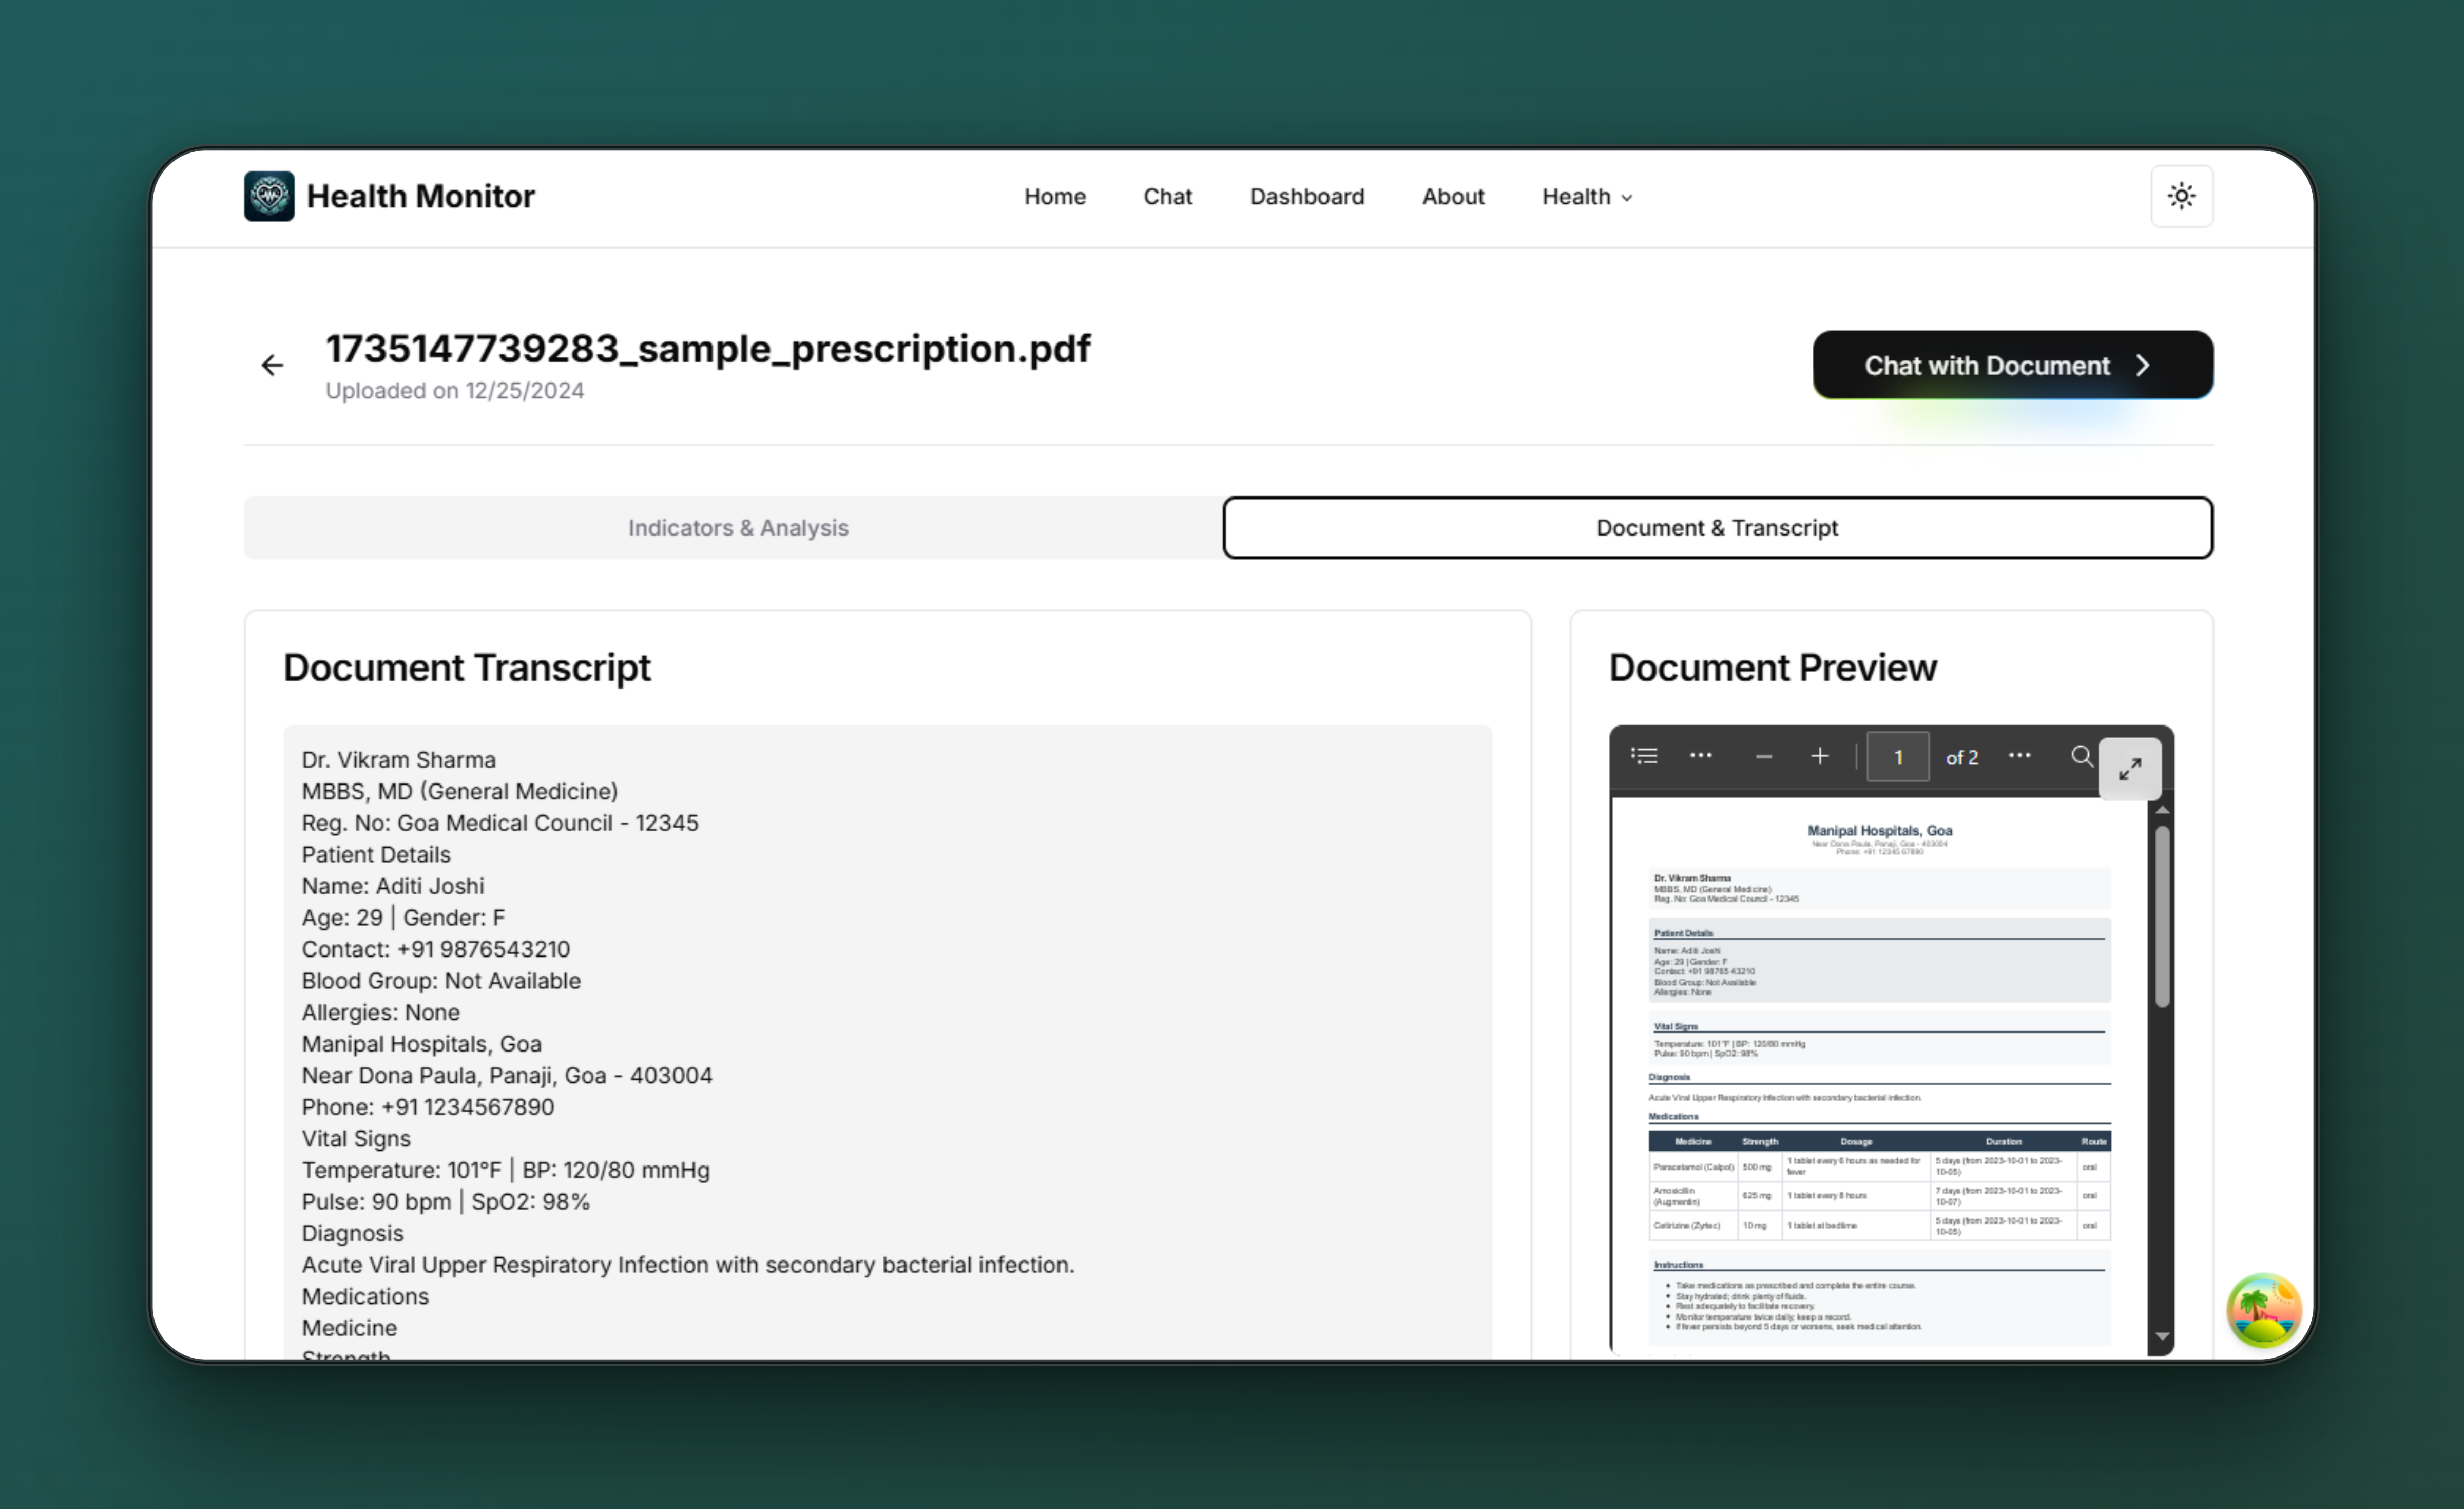
\includegraphics[width=0.8\textwidth]{public/landing/hm-record-transcript.png}
    \caption{Document Processing and Analysis Pipeline}
\end{figure}

Key components of the RAG pipeline:
\begin{enumerate}
    \item \textbf{Data Ingestion}
    \begin{itemize}
        \item Document processing (PDF, images)
        \item Sensor data integration
        \item Medical record parsing
    \end{itemize}

    \item \textbf{Data Processing}
    \begin{itemize}
        \item Text extraction and OCR
        \item Embedding generation
        \item Vector database storage
    \end{itemize}

    \item \textbf{Information Retrieval}
    \begin{itemize}
        \item Semantic search
        \item Context-aware querying
        \item Real-time data aggregation
    \end{itemize}
\end{enumerate}

\subsection{AI Integration}
\begin{figure}[H]
    \centering
    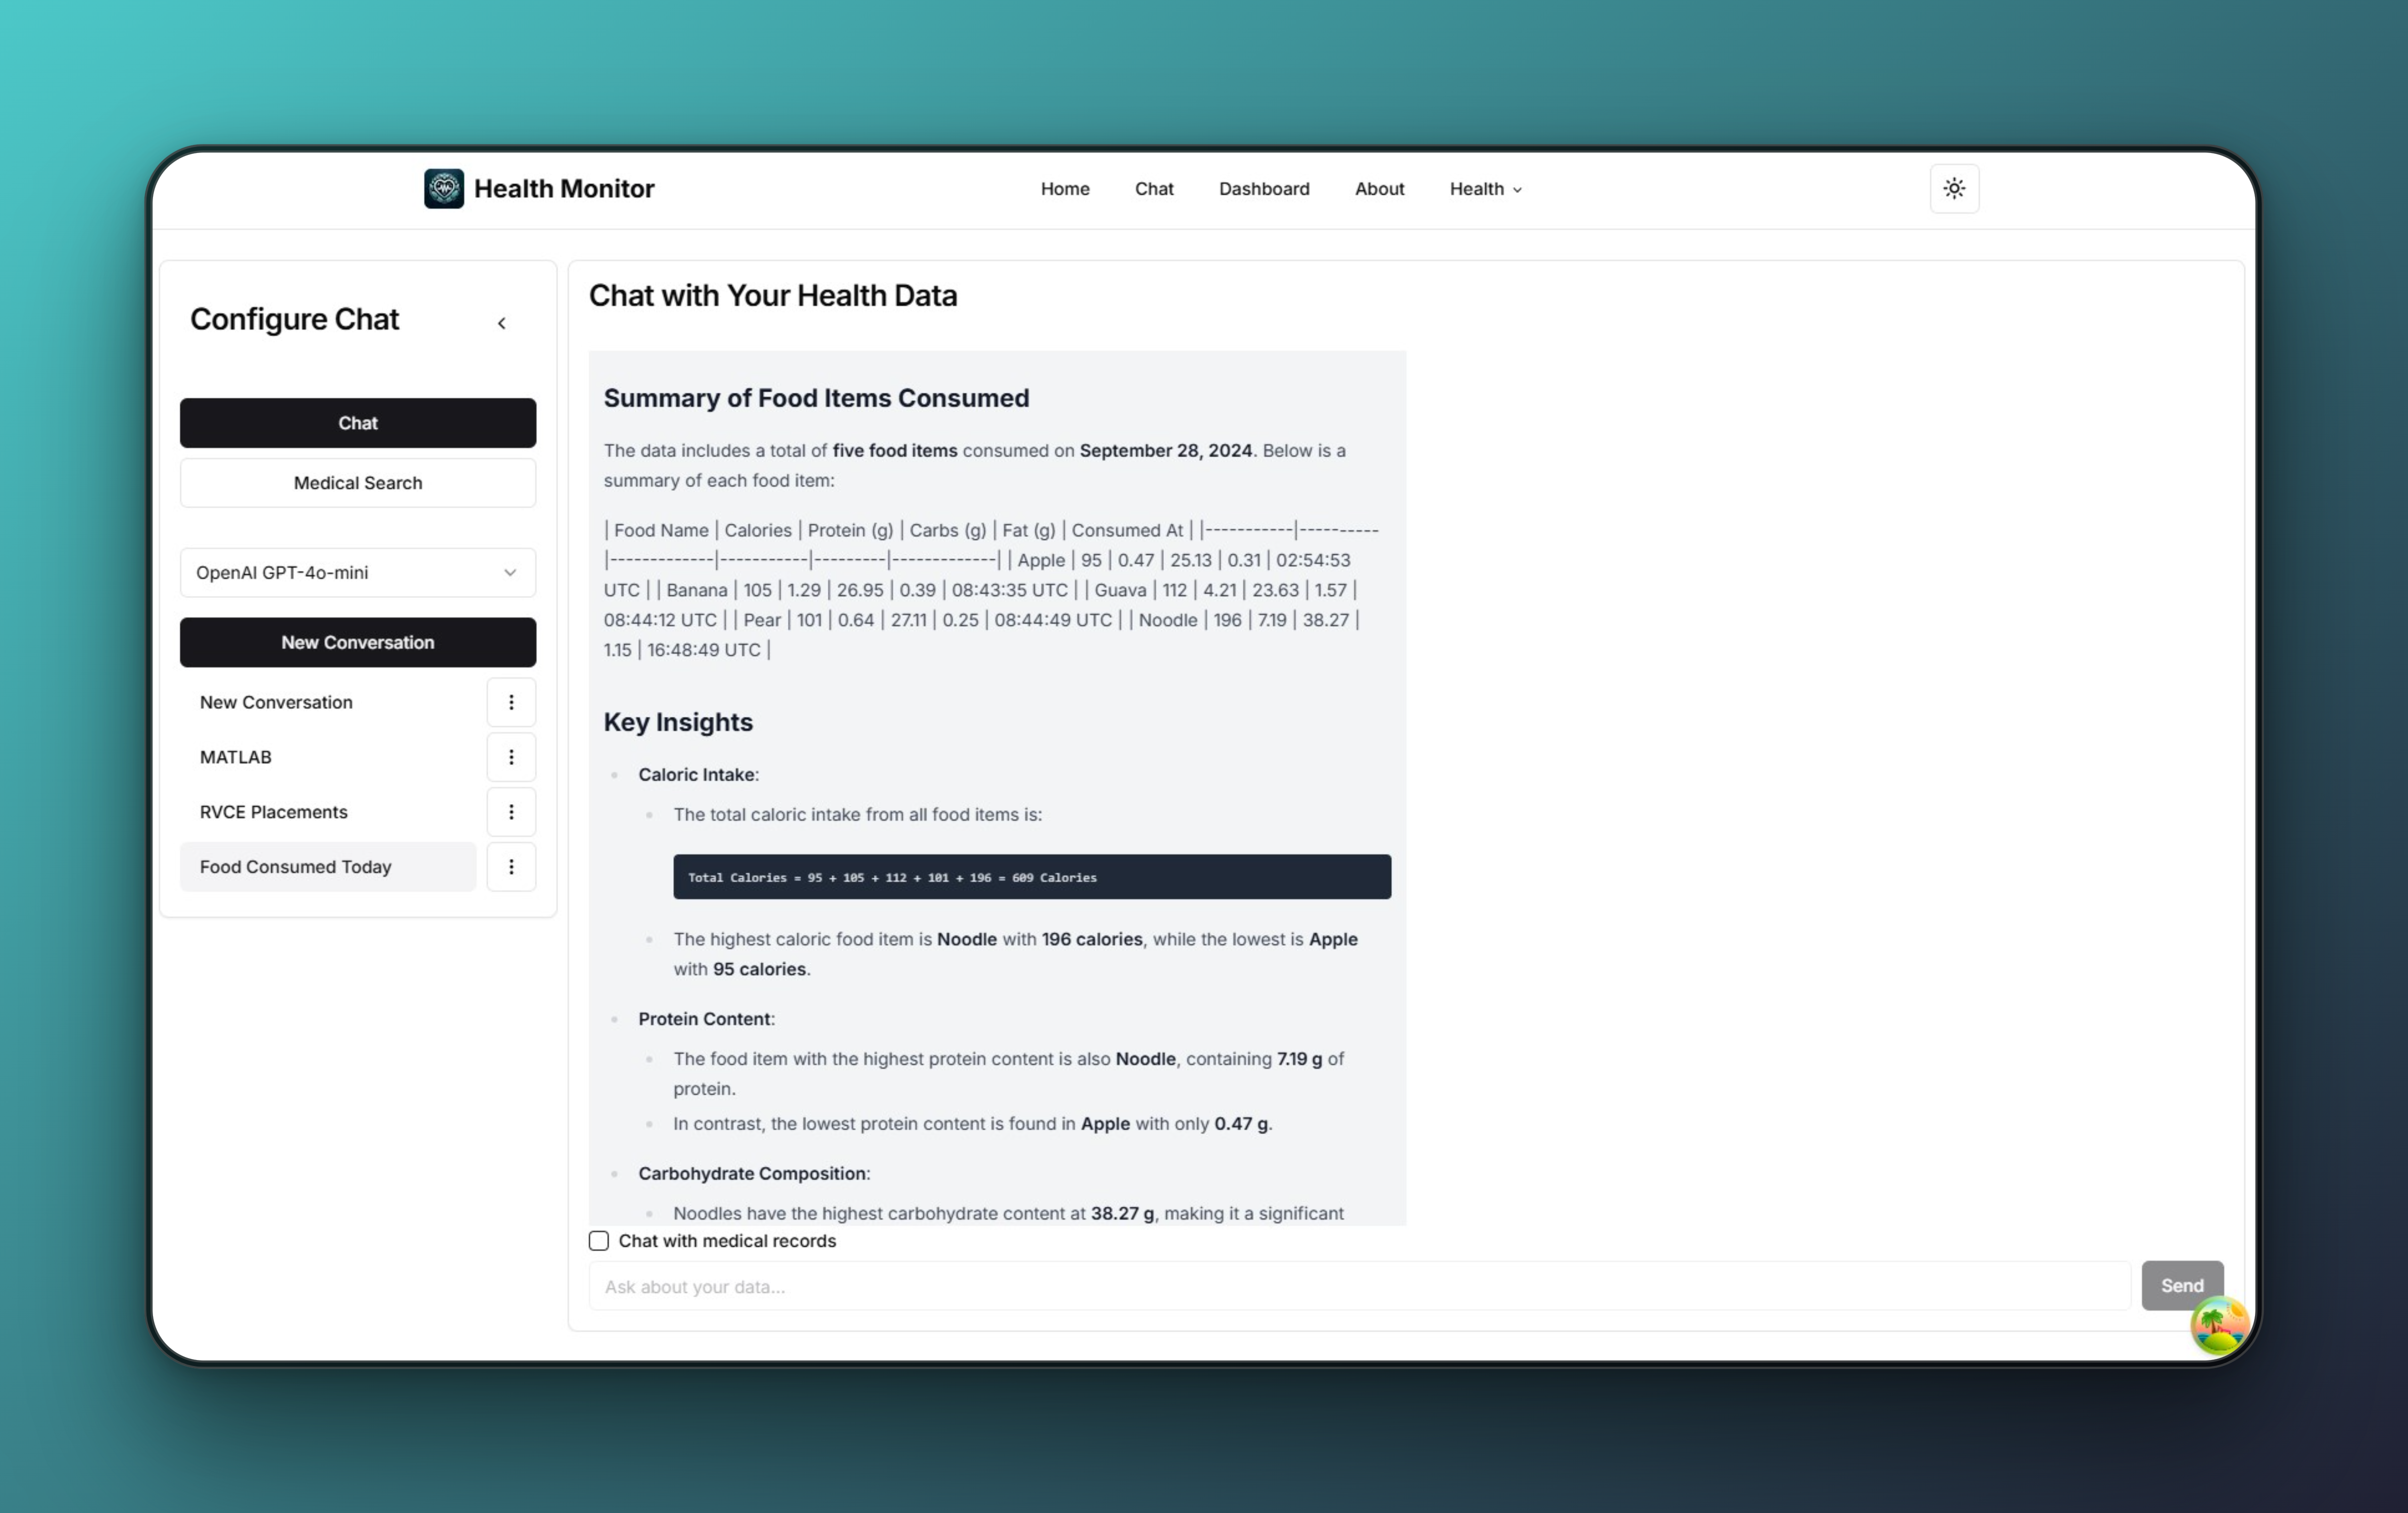
\includegraphics[width=0.8\textwidth]{public/landing/hm-chat-light.png}
    \caption{AI Health Assistant Interface}
\end{figure}

Implementation of AI features includes:
\begin{itemize}
    \item Natural language processing for user queries
    \item Context-aware response generation
    \item Medical terminology explanation
    \item Personalized health insights
\end{itemize}

\subsection{Data Visualization}
\begin{figure}[H]
    \centering
    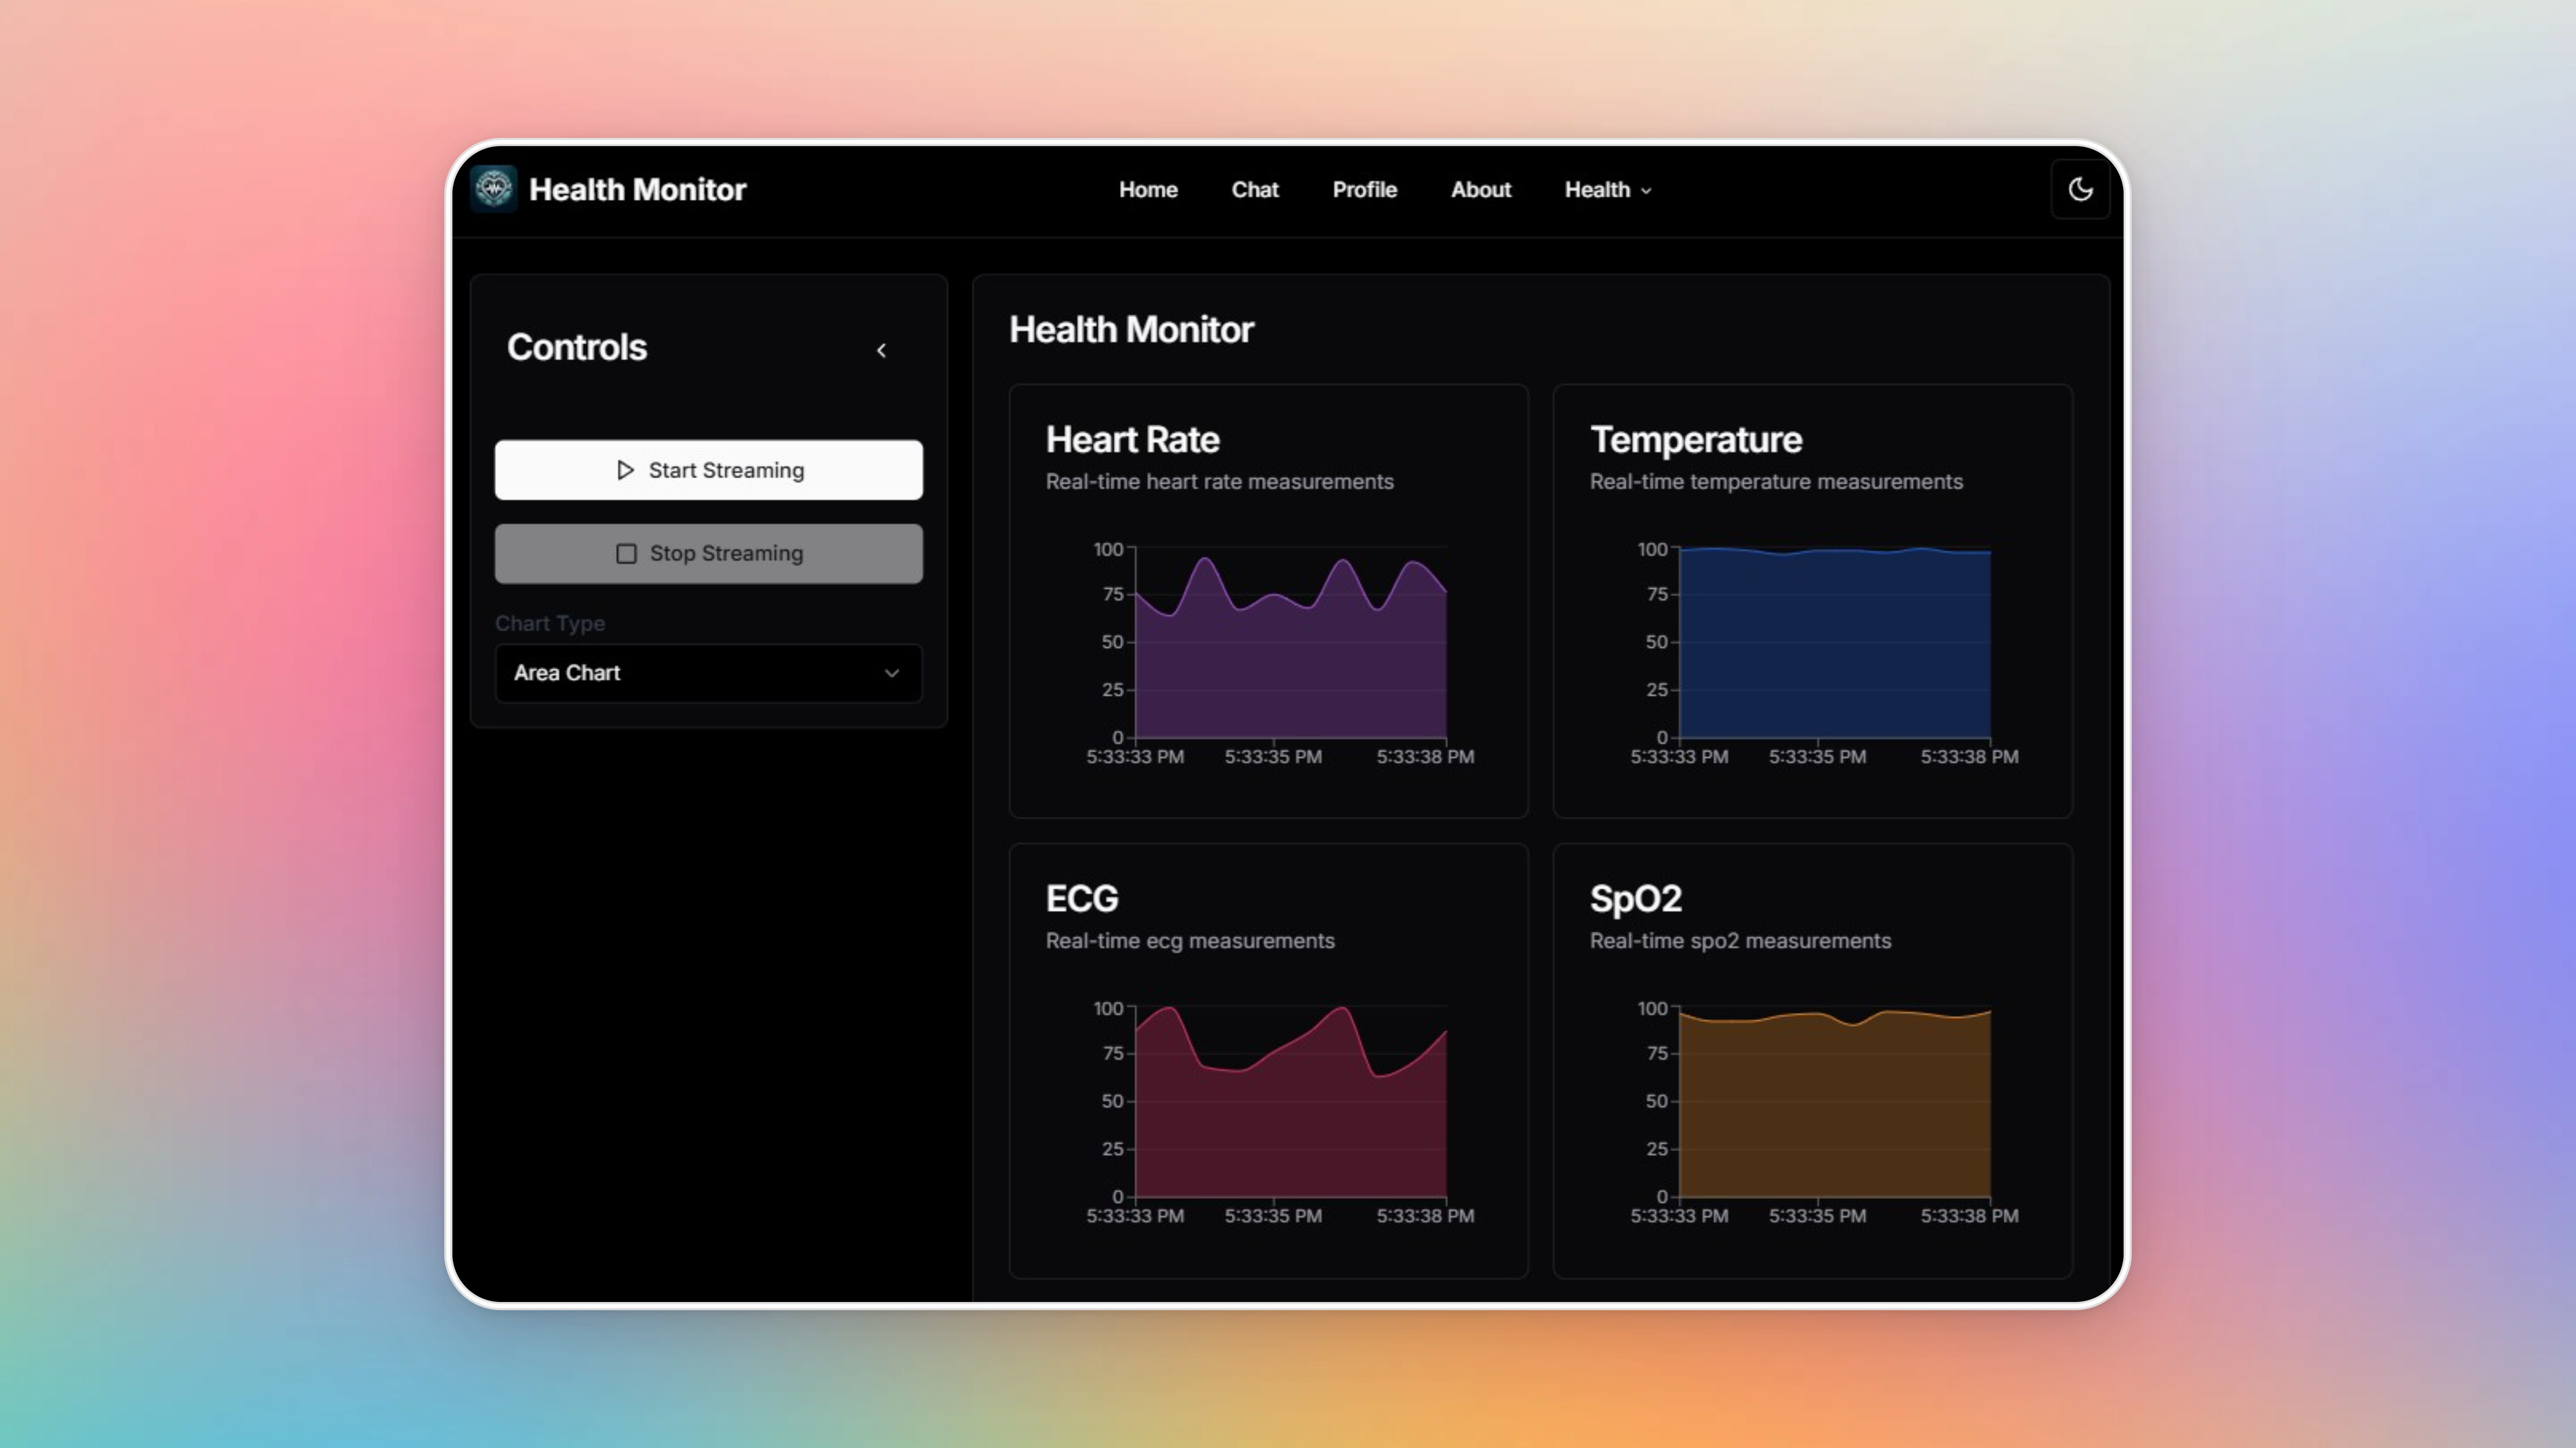
\includegraphics[width=0.8\textwidth]{public/landing/hm-graphs.png}
    \caption{Health Data Visualization Components}
\end{figure}

The visualization system includes:
\begin{itemize}
    \item Interactive charts and graphs
    \item Real-time sensor data display
    \item Health trend analysis
    \item Customizable dashboards
\end{itemize}

\subsection{Project Access}
The project can be accessed through:

\begin{itemize}
    \item GitHub Repository: \url{https://github.com/avinash-bharti/health-monitor}
    \item Live Demo: \url{https://health-monitor-demo.vercel.app}
    \item Documentation: Available in the repository's README
\end{itemize}

\section{Interface Screenshots}
The following screenshots showcase various aspects of the implemented prototype:

\subsection{Landing Page}
\begin{figure}[H]
    \centering
    \includegraphics[width=0.45\textwidth]{public/landing/hm-landing-new.png}
    \caption{HealthHub Main Landing Page}
\end{figure}

\subsection{Health Assistant Interface}
\begin{figure}[H]
    \centering
    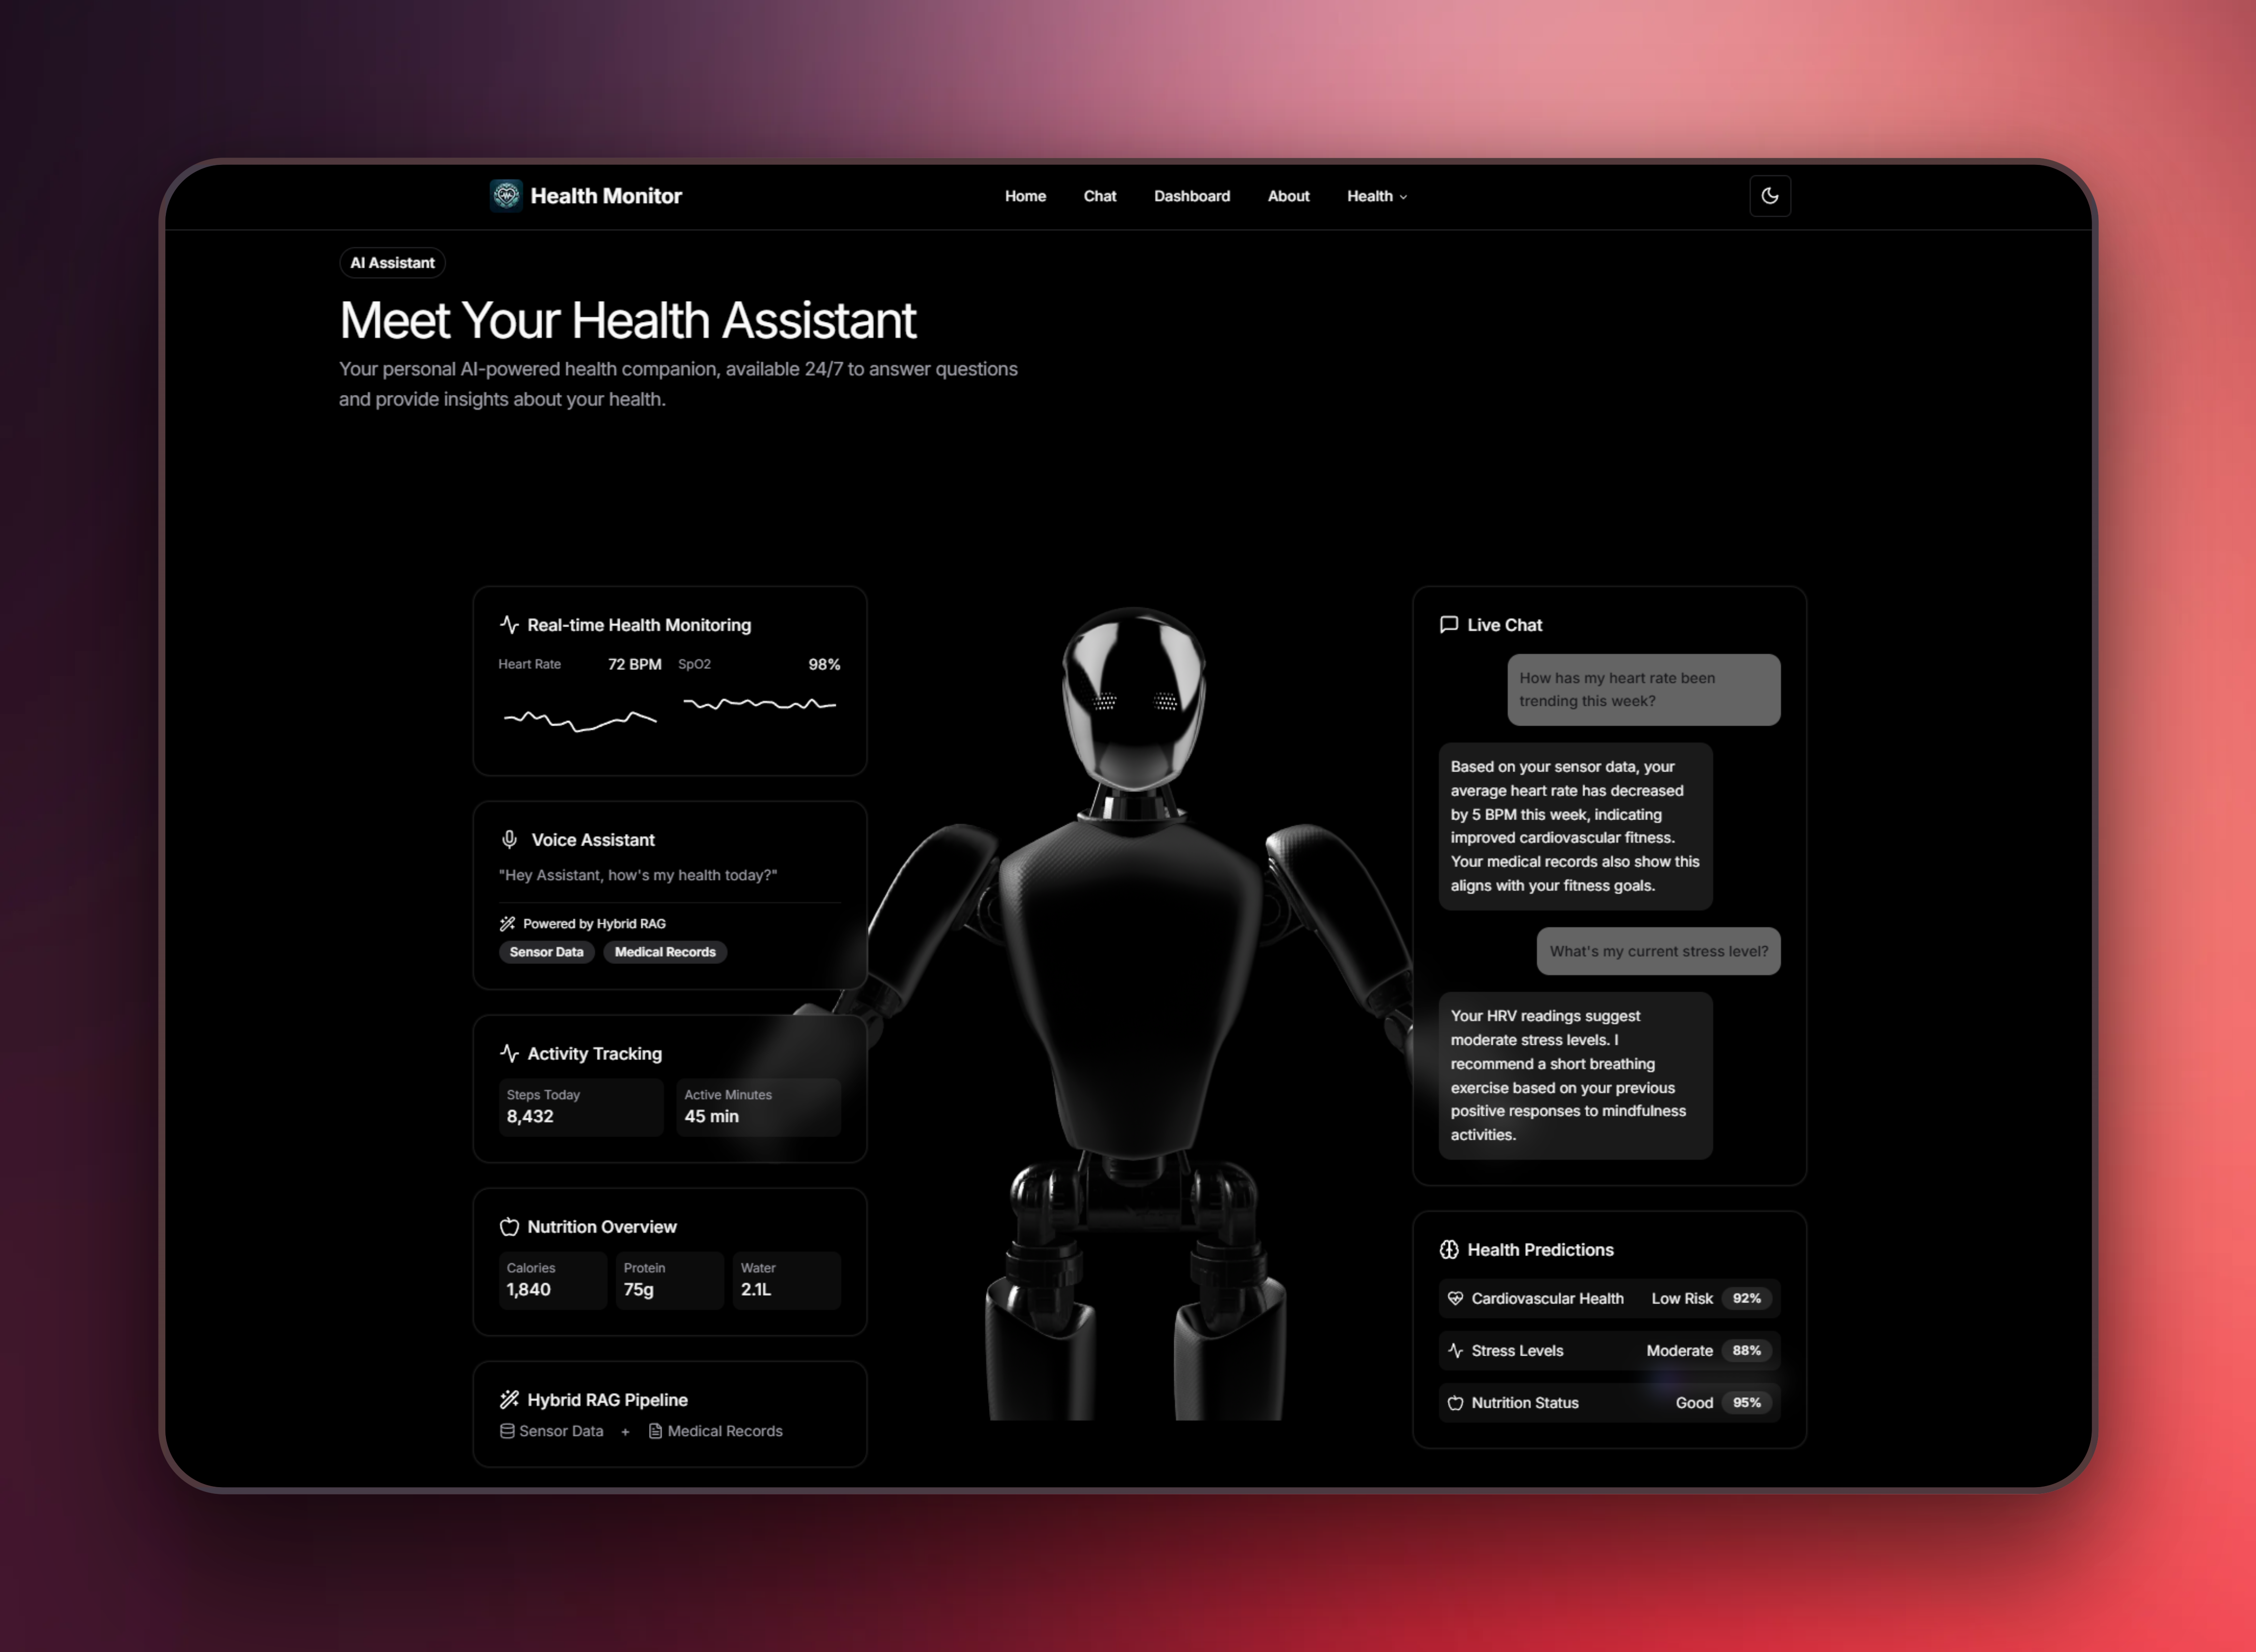
\includegraphics[width=0.45\textwidth]{public/landing/hm-landing-health-assistant-3.png}
    \caption{AI-Powered Health Assistant}
\end{figure}

\subsection{Dashboard and Analytics}
\begin{figure}[H]
    \centering
    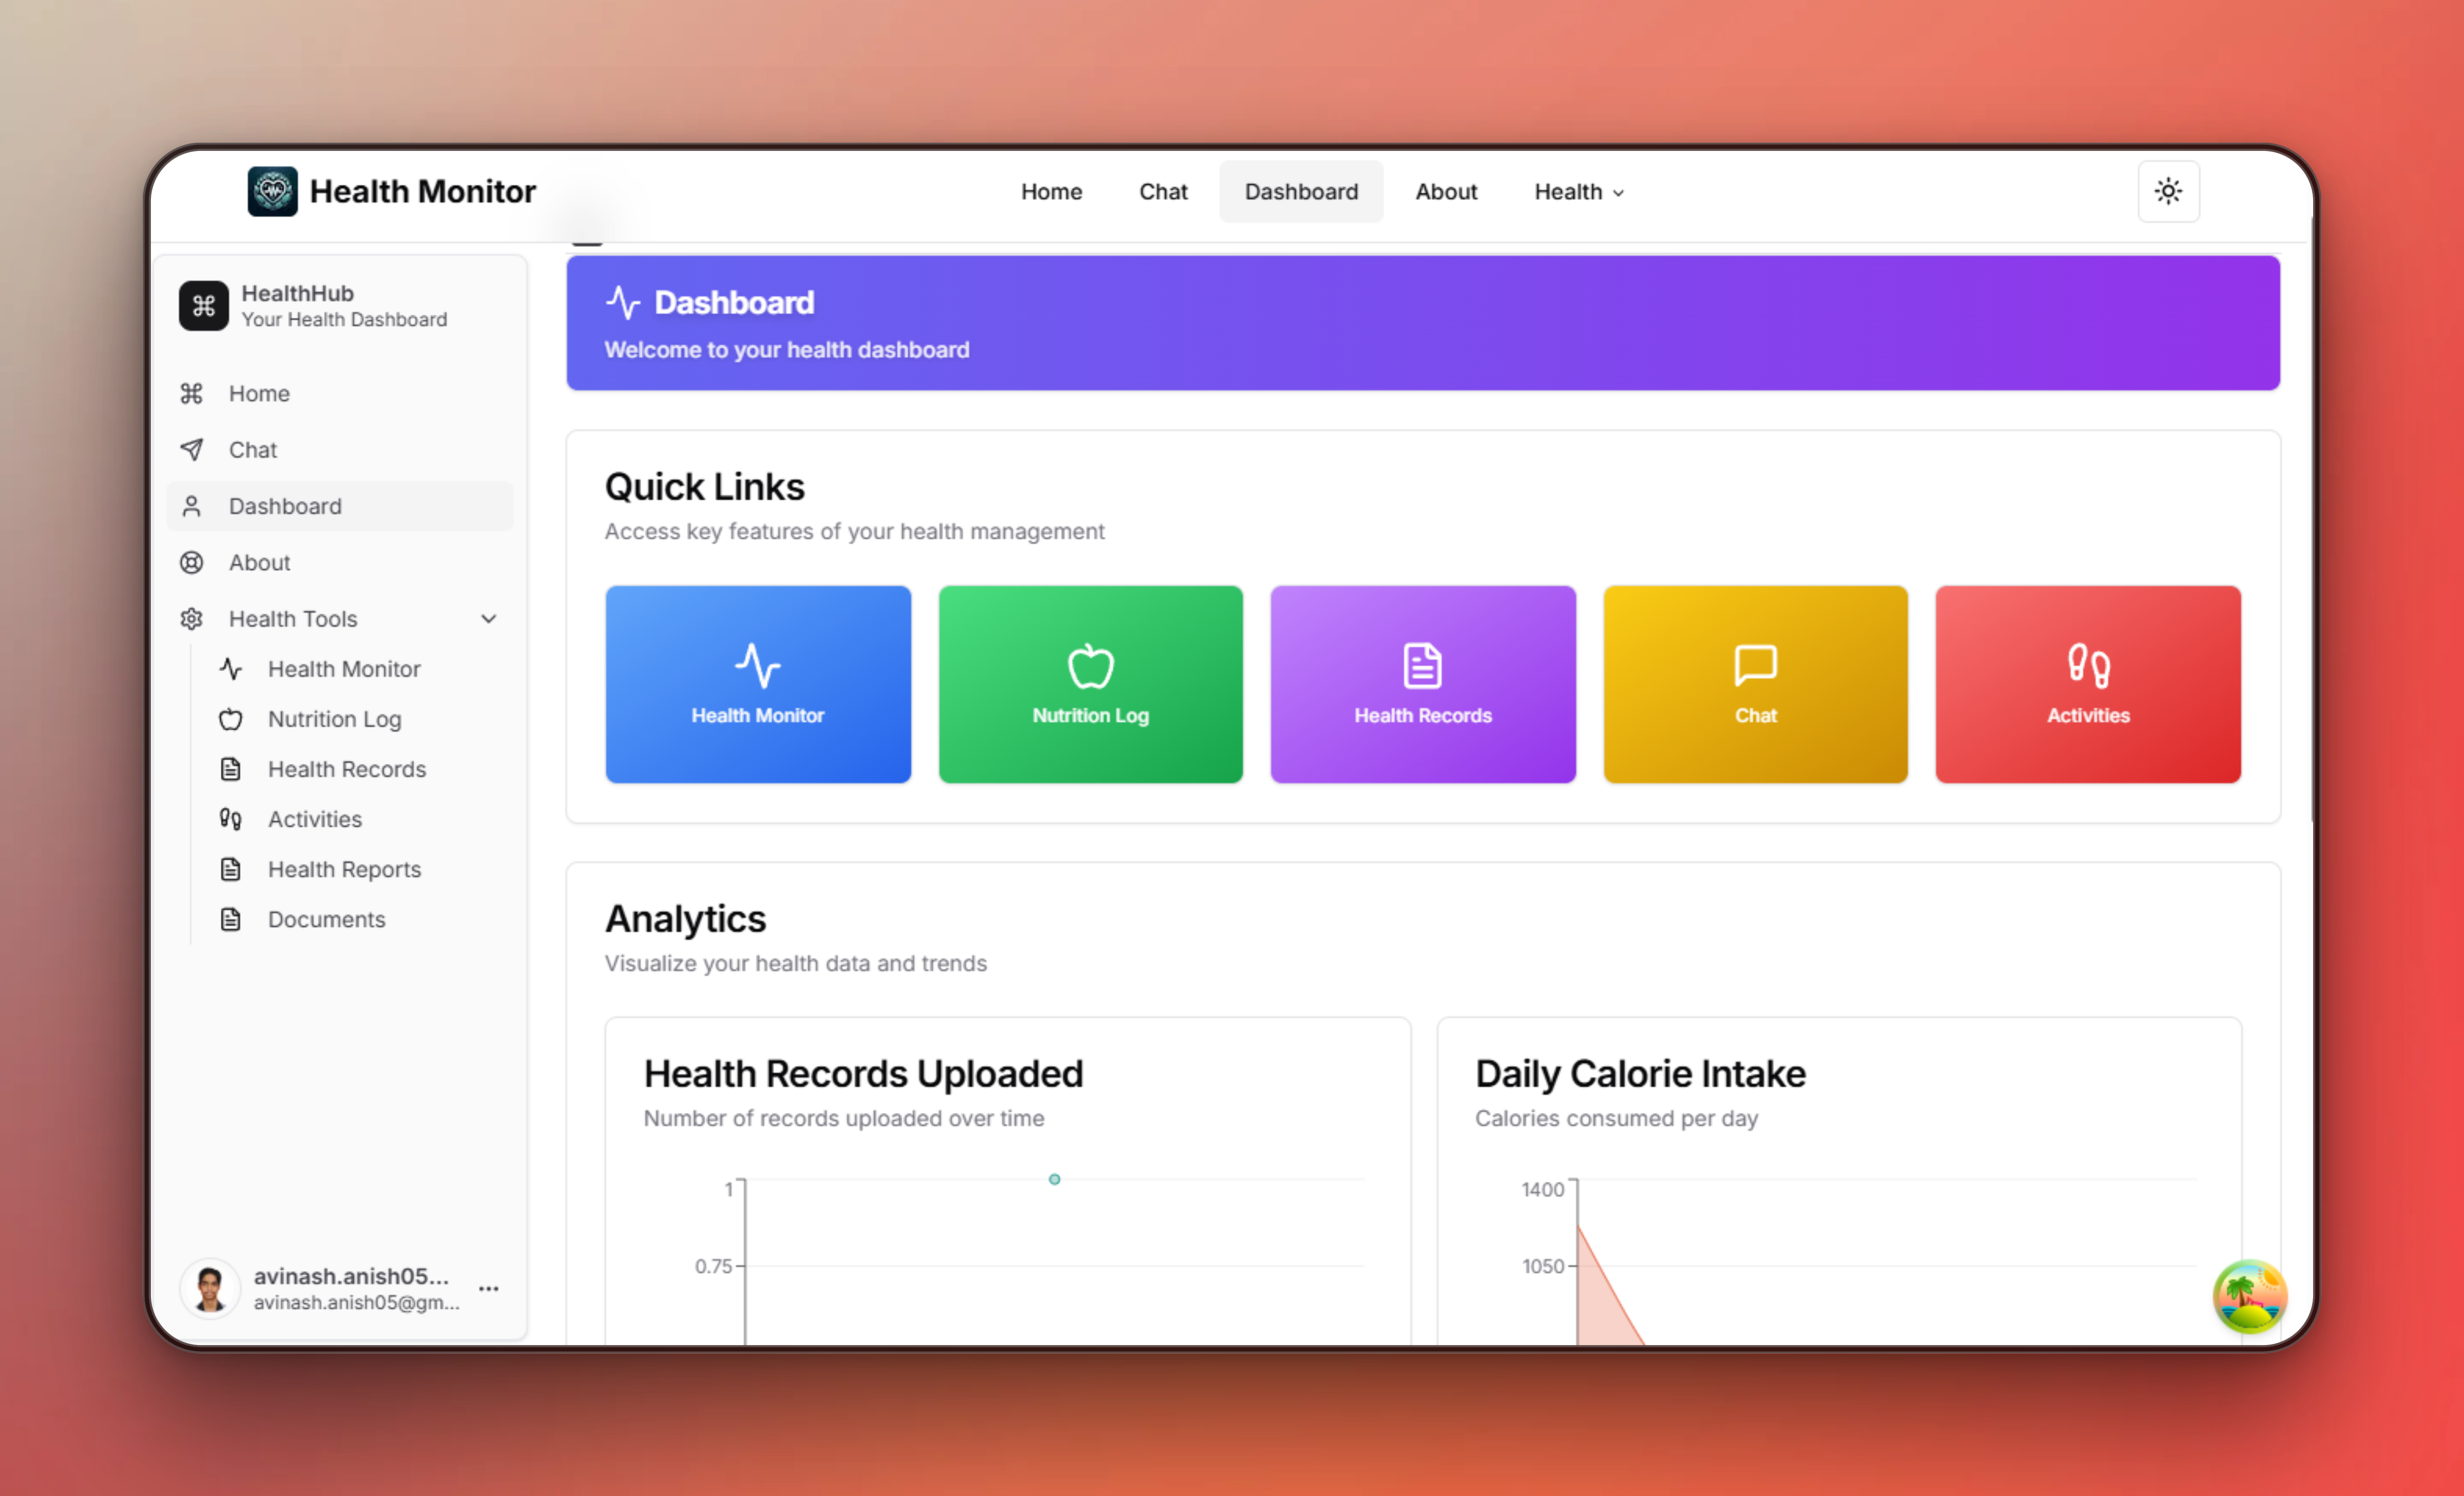
\includegraphics[width=0.45\textwidth]{public/landing/hm-dashboard.png}
    \caption{Interactive Dashboard Interface}
\end{figure}

\subsection{Data Visualization}
\begin{figure}[H]
    \centering
    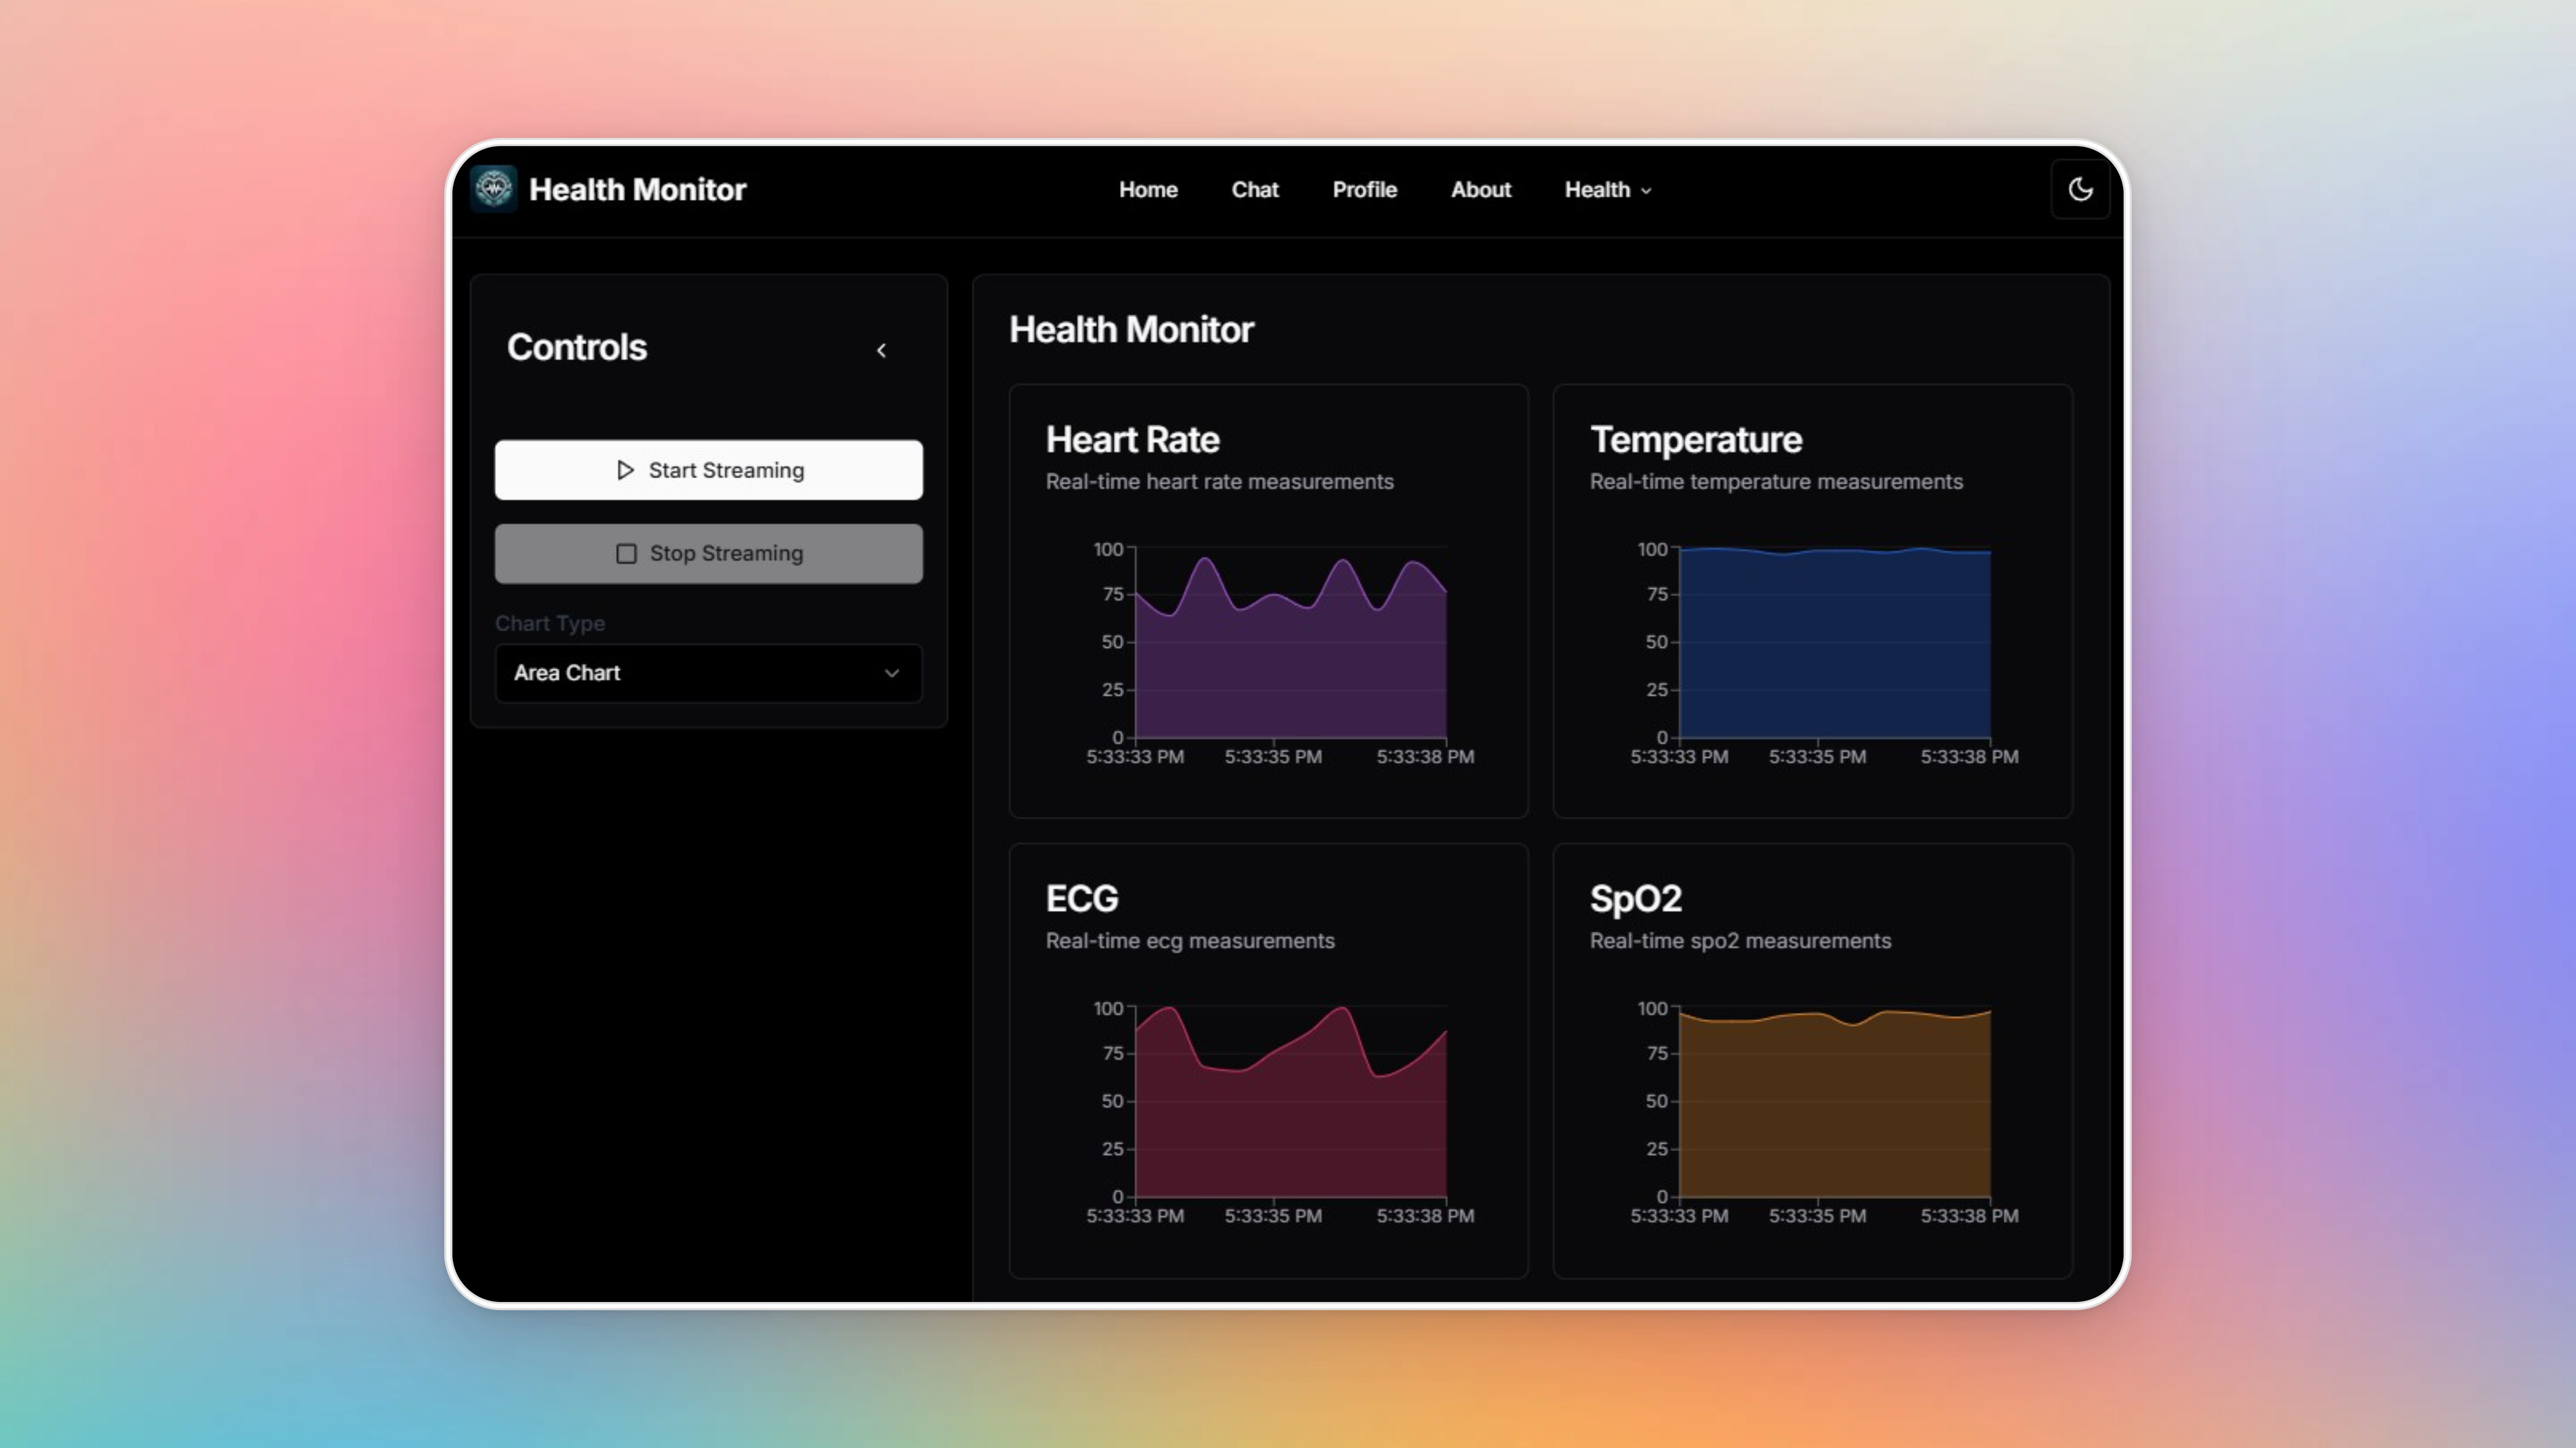
\includegraphics[width=0.45\textwidth]{public/landing/hm-graphs.png}
    \caption{Health Data Analytics and Visualization}
\end{figure}

\subsection{Record Management}
\begin{figure}[H]
    \centering
    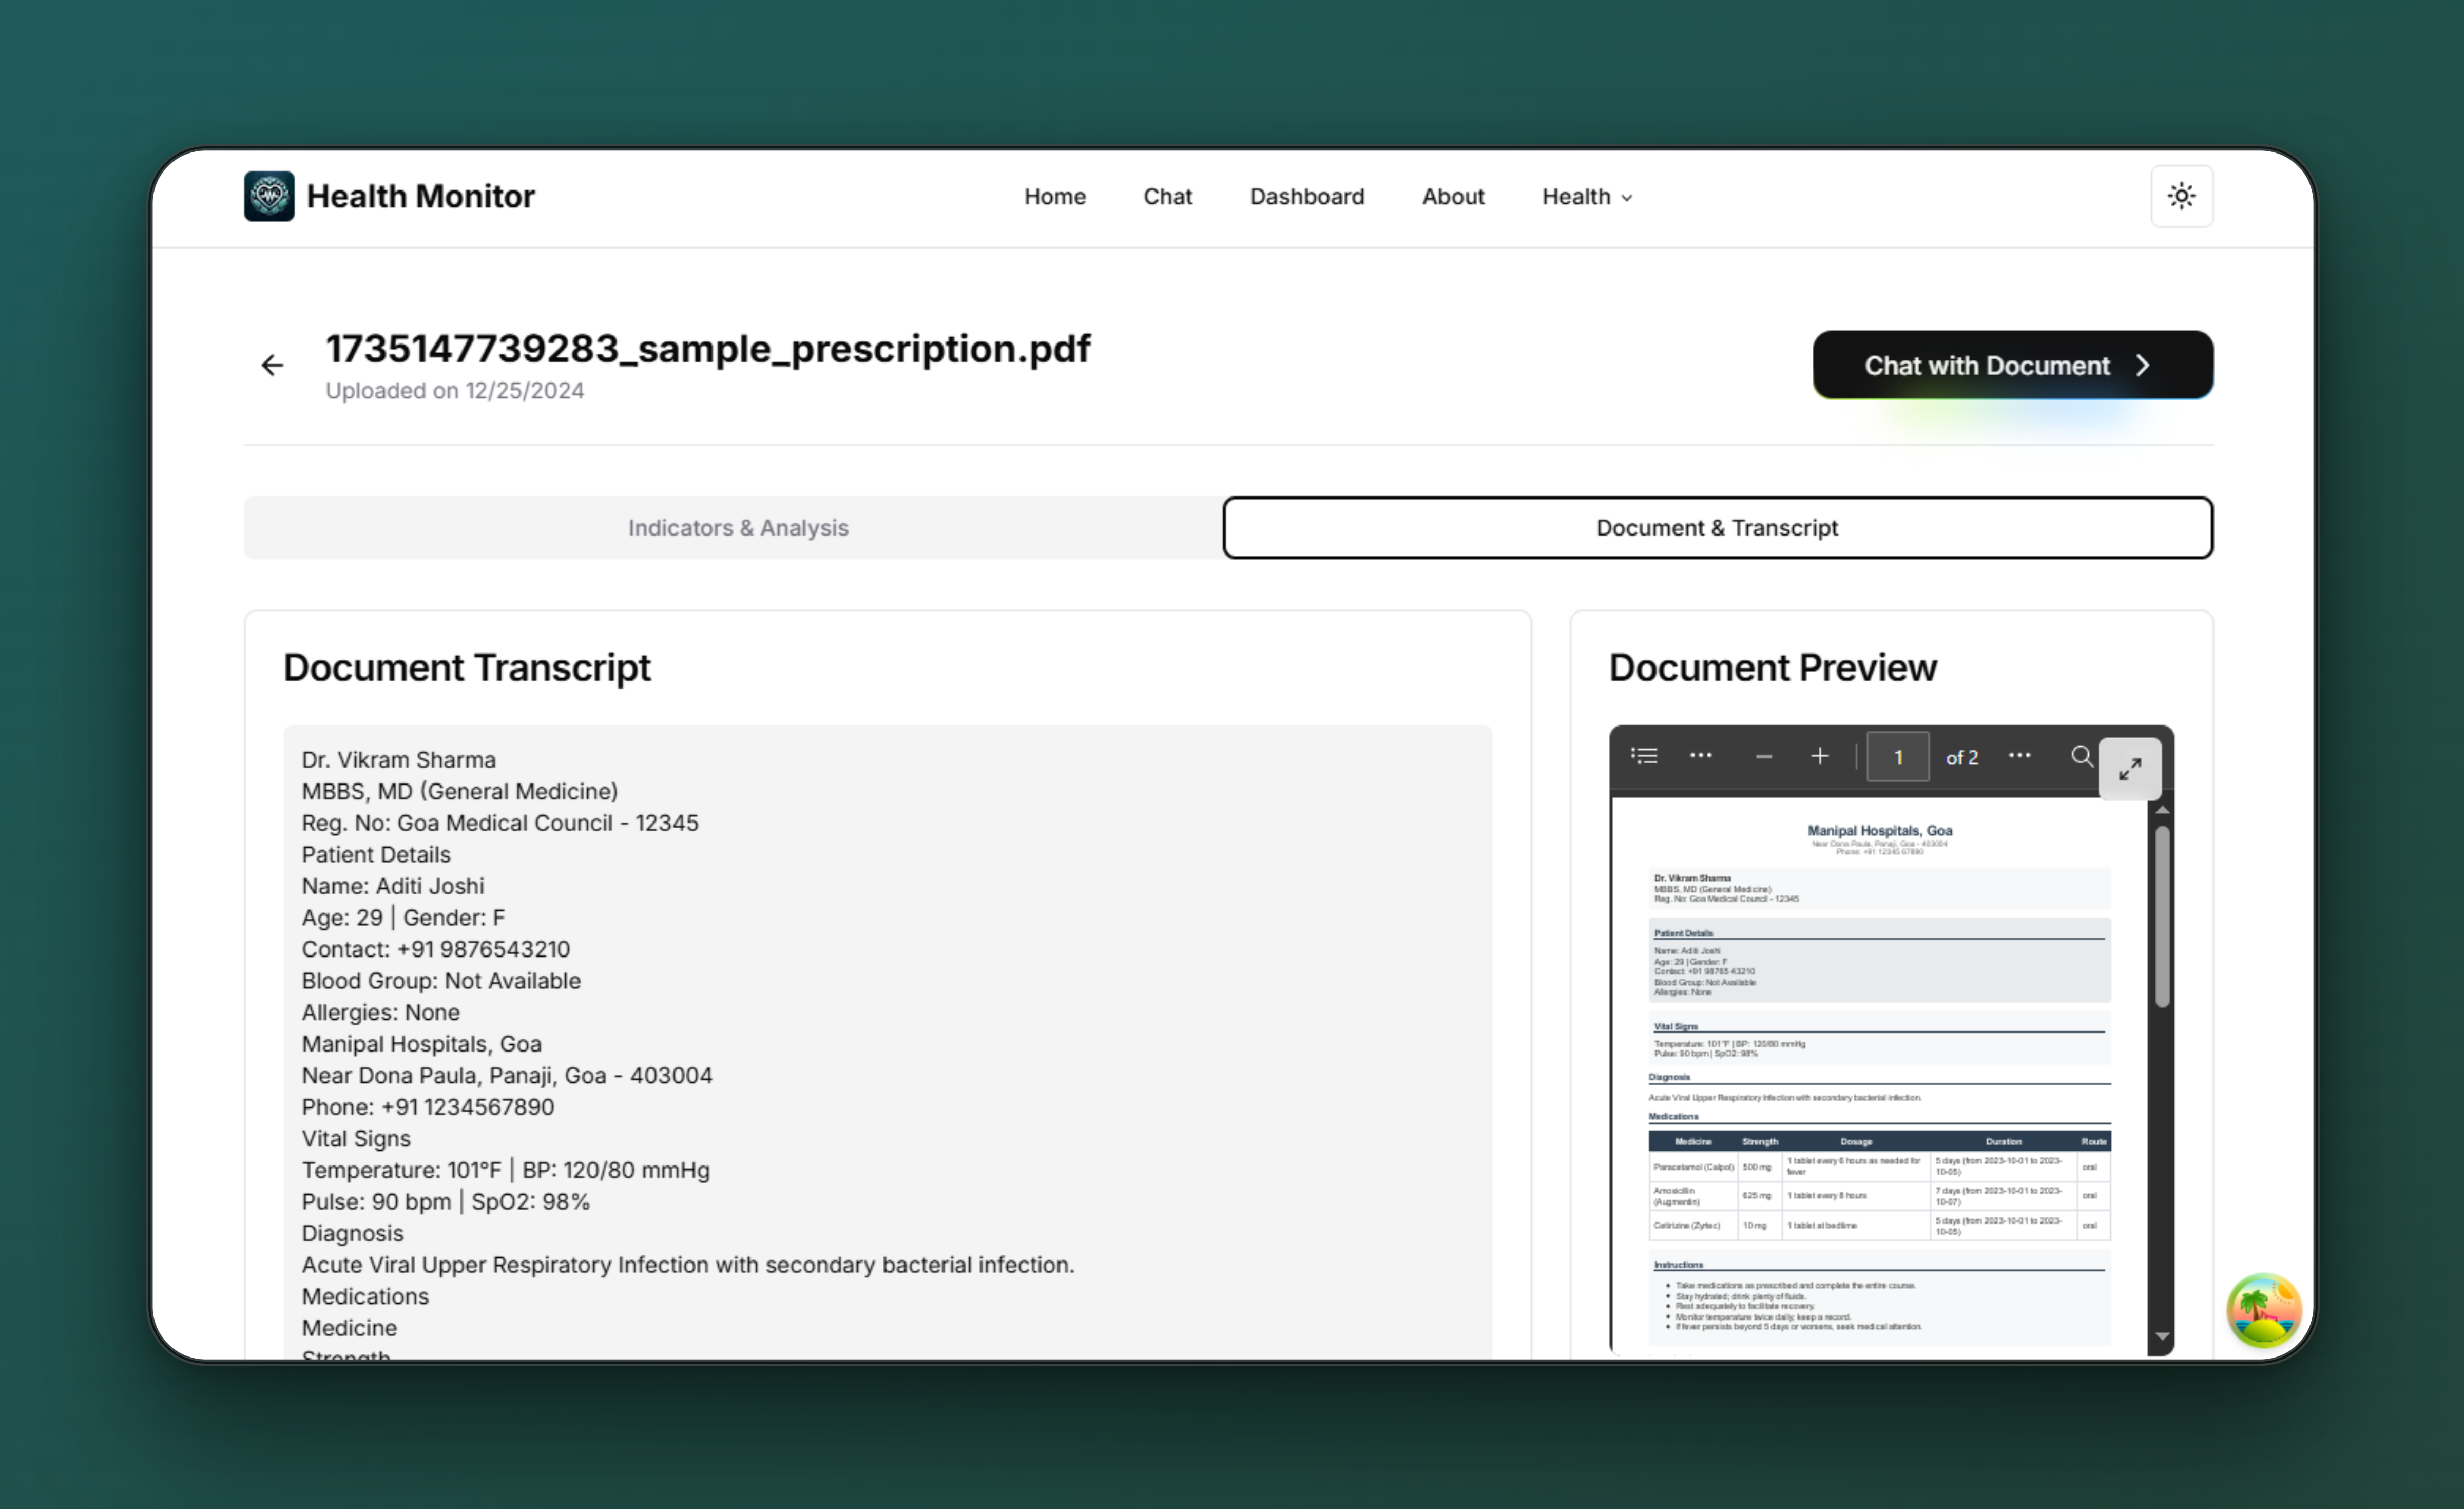
\includegraphics[width=0.45\textwidth]{public/landing/hm-record-transcript.png}
    \caption{Medical Record Processing Interface}
\end{figure}

\subsection{Analysis Reports}
\begin{figure}[H]
    \centering
    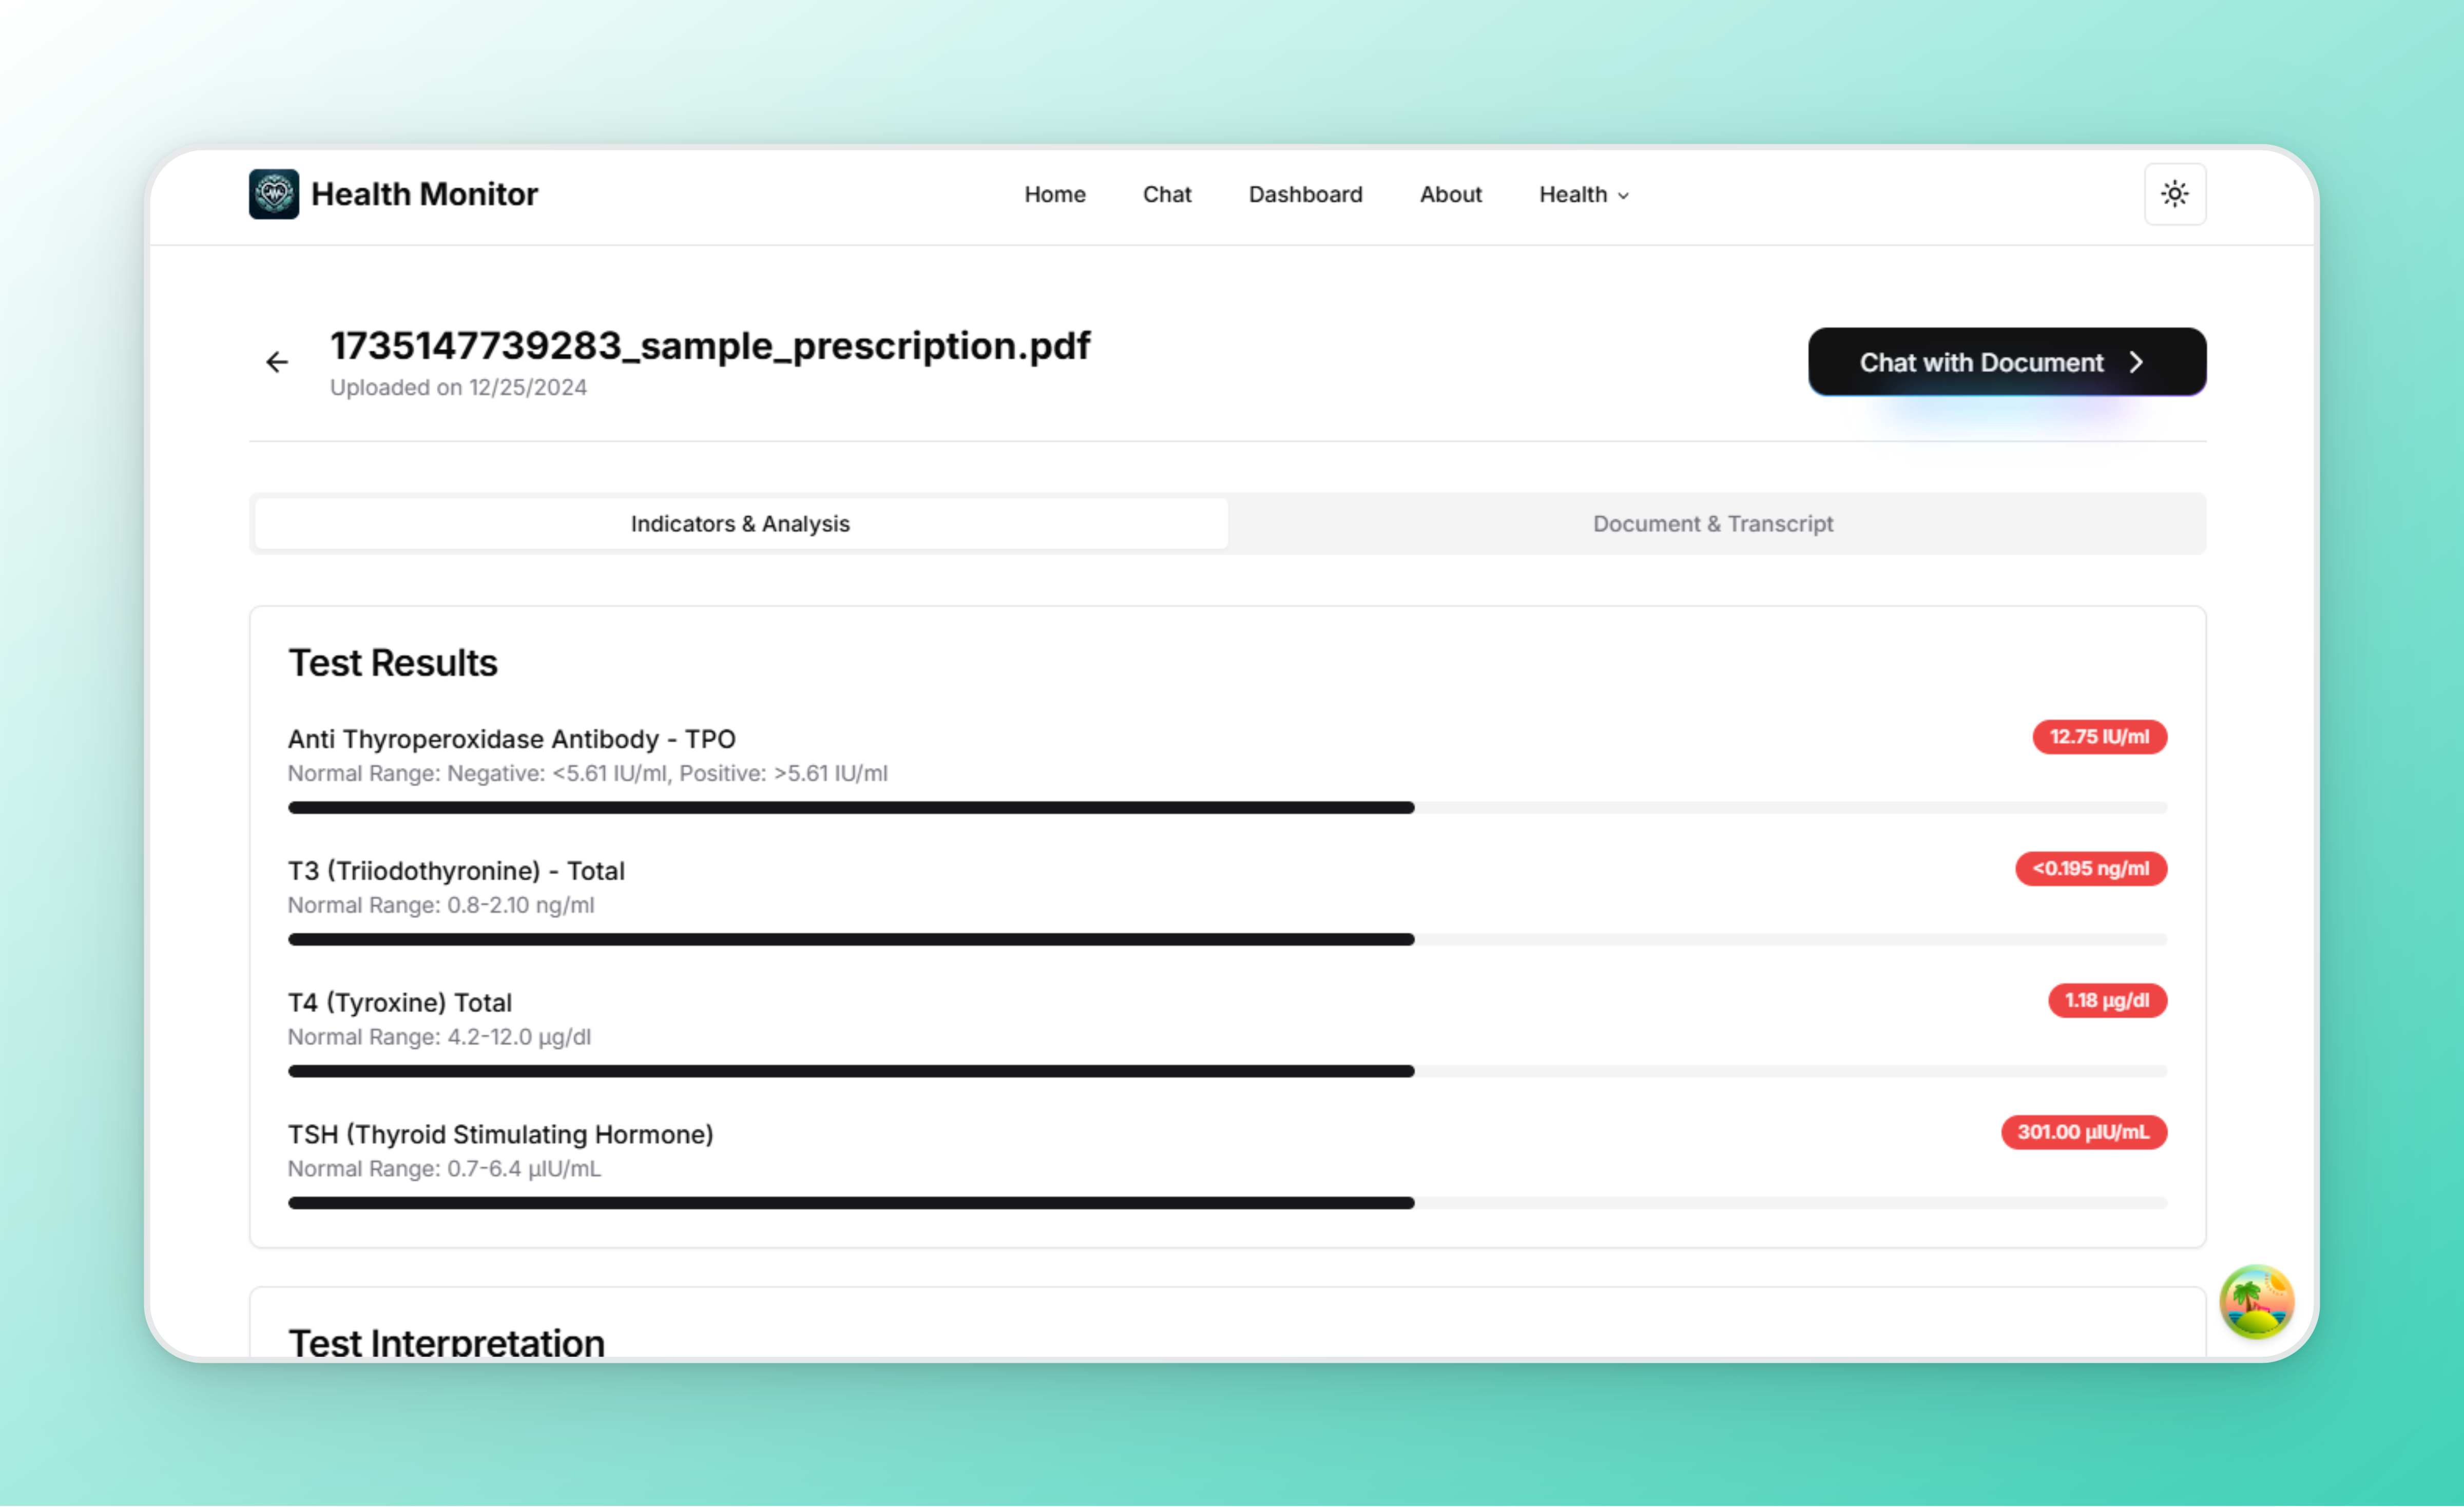
\includegraphics[width=0.45\textwidth]{public/landing/hm-record-analysis.png}
    \caption{Health Record Analysis View}
\end{figure}

\subsection{Activity Tracking}
\begin{figure}[H]
    \centering
    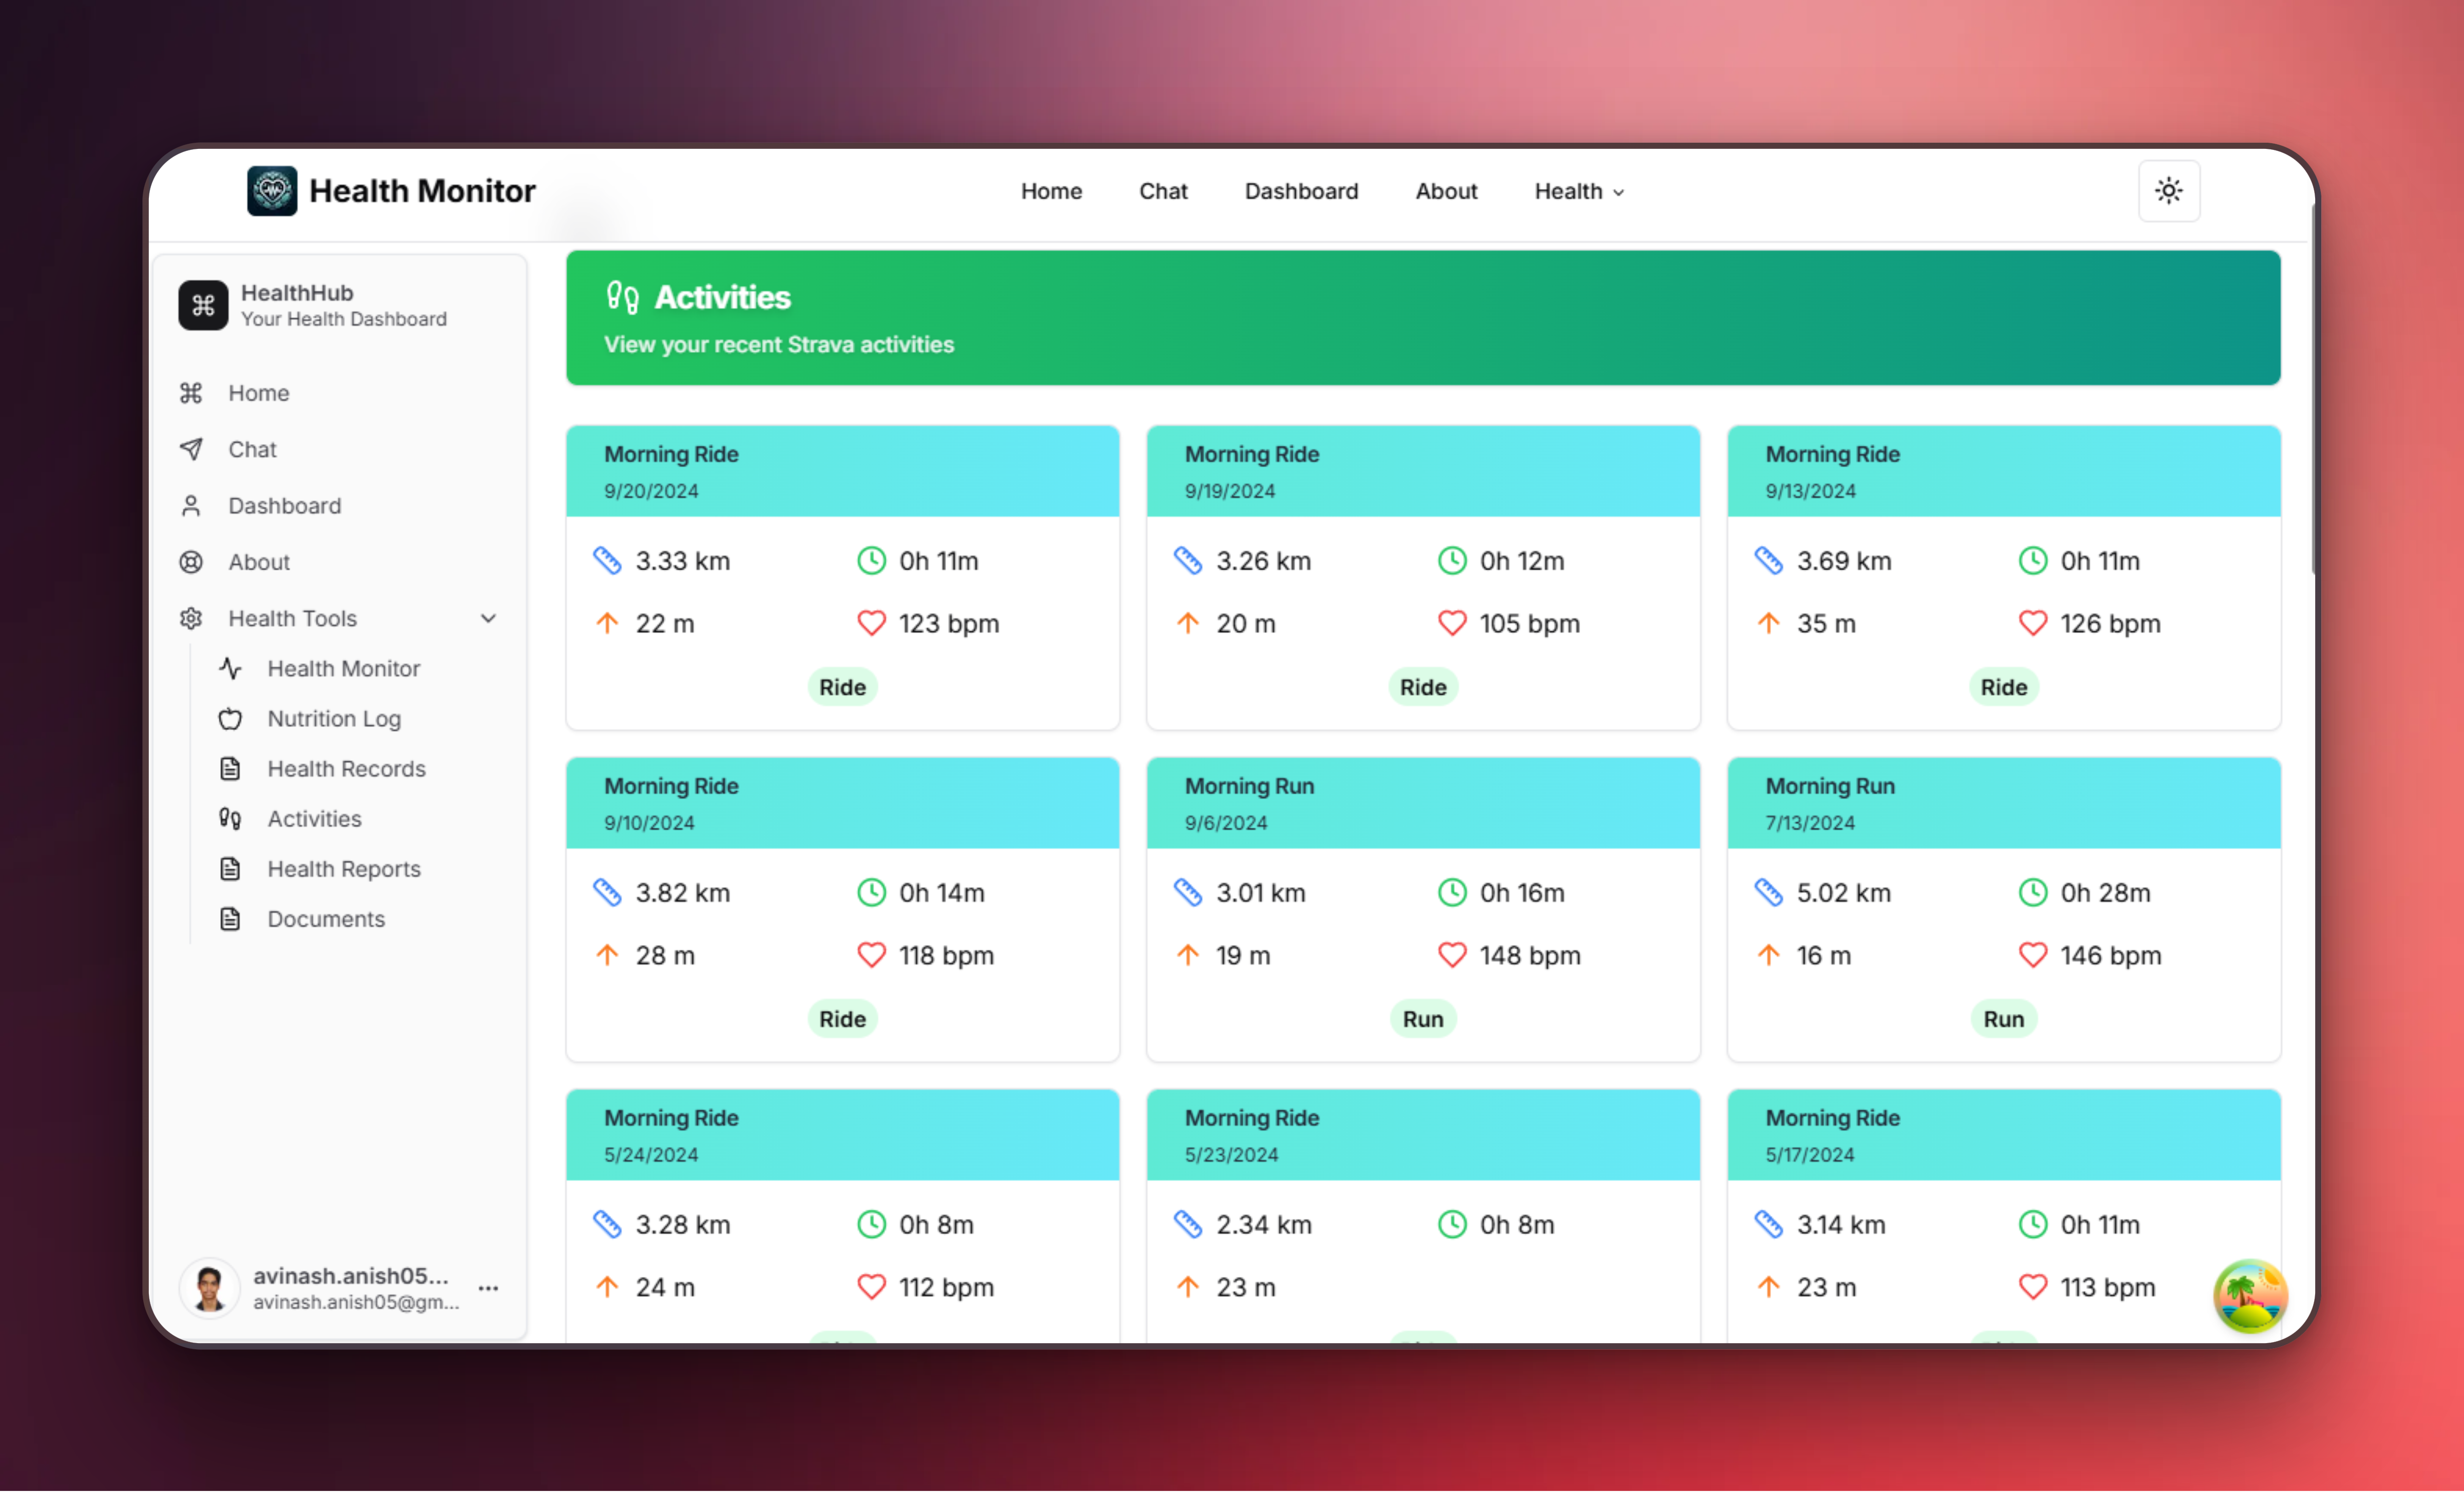
\includegraphics[width=0.45\textwidth]{public/landing/hm-activities.png}
    \caption{Physical Activity Monitoring Interface}
\end{figure}

\subsection{Nutrition Tracking}
\begin{figure}[H]
    \centering
    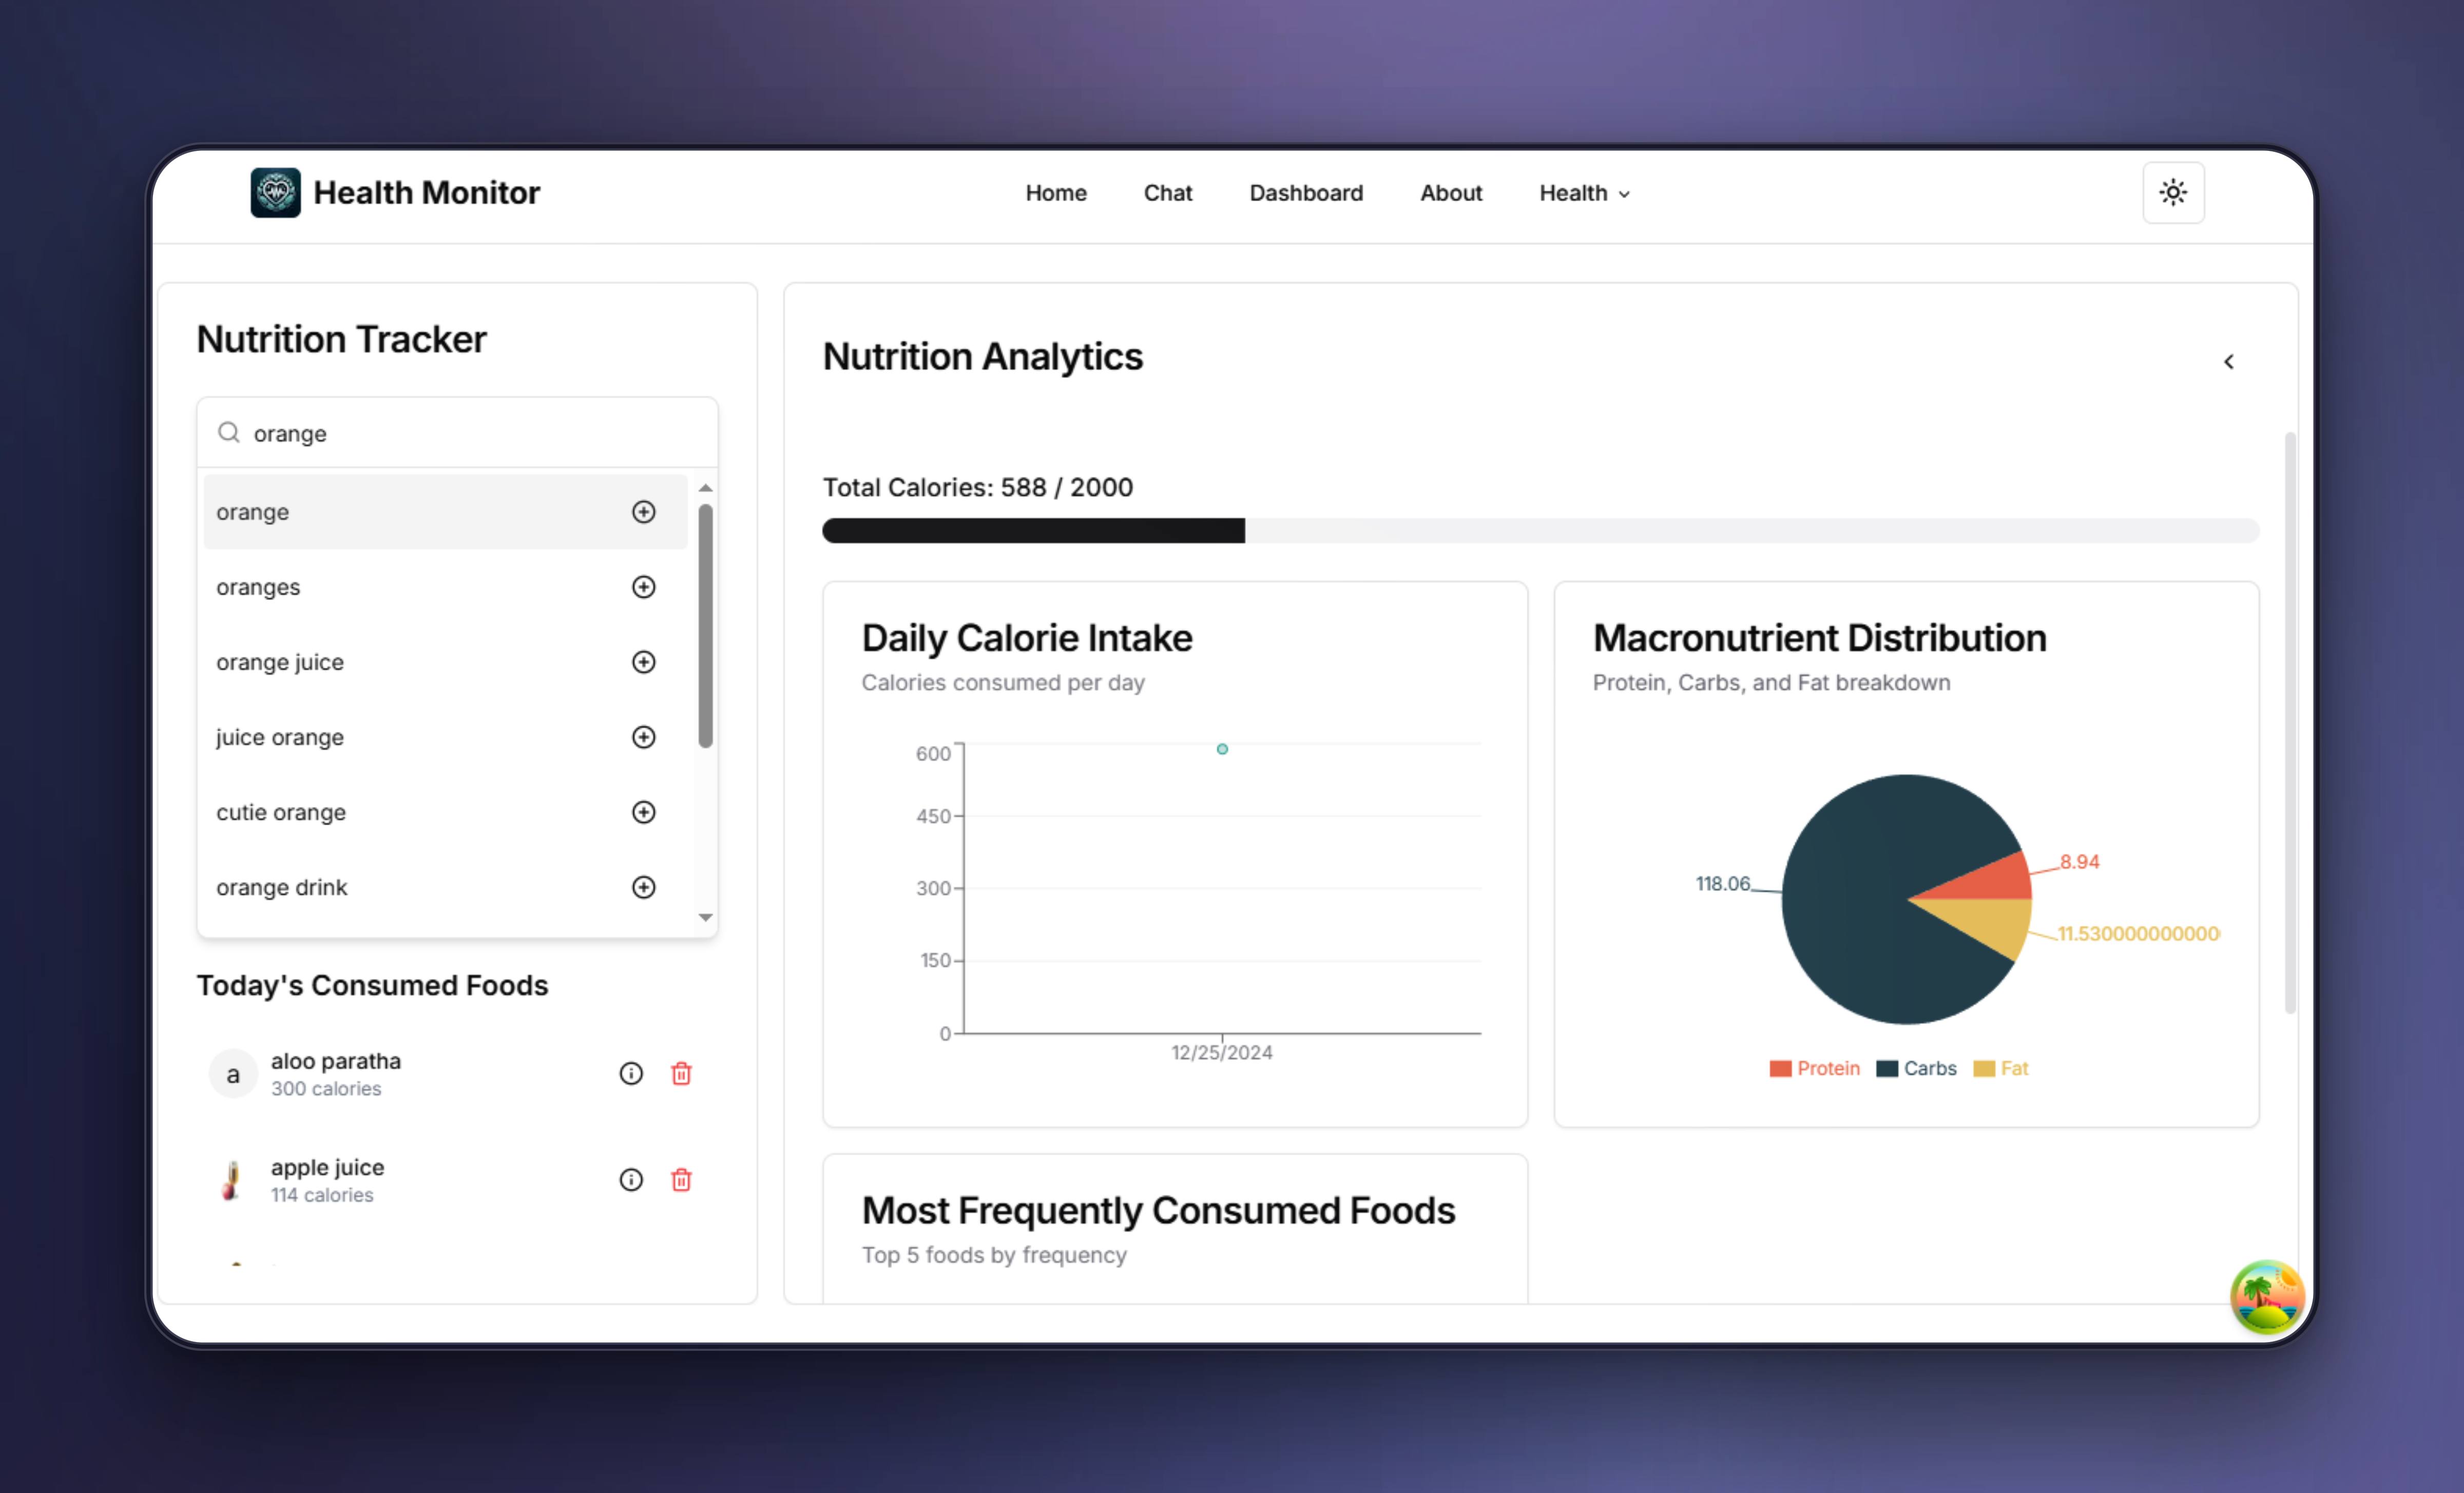
\includegraphics[width=0.45\textwidth]{public/landing/hm-nutrition.png}
    \caption{Nutrition Monitoring and Analysis}
\end{figure}

\section{Example Use Cases and Workflow}
\subsection{Example Queries and Responses}

To demonstrate the system's capabilities, here are some example interactions:

\begin{tcolorbox}[title=Query 1: Complex Medical History]
\textbf{User:} "What medications was I prescribed after my surgery last year, and how did they interact with my current heart condition?"

\textbf{System Response:}
\begin{itemize}
    \item Post-surgery medications: Tramadol (pain), Cephalexin (antibiotic)
    \item Current heart condition: Atrial fibrillation
    \item Interaction found: Tramadol noted to increase heart rate
    \item Recommendation: Switch to Acetaminophen
\end{itemize}

\textbf{Sources:}
\begin{itemize}
    \item Current heart rate: 72 bpm (sensor data)
    \item Surgical Report (07/15/2023)
    \item Cardiology Follow-up (08/02/2023)
\end{itemize}
\end{tcolorbox}

\begin{tcolorbox}[title=Query 2: Data Integration]
\textbf{User:} "How has my blood pressure changed since starting the new medication?"

\textbf{System Response:}
\begin{itemize}
    \item Pre-medication average: 145/90 mmHg
    \item Current average: 128/82 mmHg
    \item 12\% improvement in systolic pressure
    \item 720 sensor readings over 30 days
\end{itemize}
\end{tcolorbox}

\subsection{System Workflow}
The implementation follows a structured workflow for processing health data:

\subsubsection{Document Processing Pipeline}
\begin{enumerate}
    \item \textbf{Document Upload}
    \begin{itemize}
        \item User uploads medical records
        \item Frontend validates format and size
        \item Secure storage in Supabase
    \end{itemize}

    \item \textbf{Text Extraction}
    \begin{itemize}
        \item OCR processing using Tesseract
        \item Text cleaning and preprocessing
        \item Medical entity recognition
    \end{itemize}

    \item \textbf{Embedding Generation}
    \begin{itemize}
        \item Text chunking for processing
        \item Vector embedding via Cohere
        \item Storage in pgvector database
    \end{itemize}
\end{enumerate}

\subsubsection{Query Processing Flow}
\begin{enumerate}
    \item \textbf{Query Input}
    \begin{itemize}
        \item Natural language query reception
        \item Query embedding generation
        \item Context retrieval initiation
    \end{itemize}

    \item \textbf{Data Retrieval}
    \begin{itemize}
        \item Vector similarity search
        \item Real-time sensor data integration
        \item Structured data querying
    \end{itemize}

    \item \textbf{Response Generation}
    \begin{itemize}
        \item Context assembly
        \item LLM processing
        \item Response formatting and validation
    \end{itemize}
\end{enumerate}  % Prototyping chapter
\pagestyle{fancy}
\thispagestyle{fancy}
\chapter{Testing}
\section{Introduction to Testing}
Our testing strategy encompassed multiple layers of validation to ensure the reliability, security, and usability of the HealthHub platform. We implemented a comprehensive testing approach that covered both technical functionality and user experience.

\section{Types of testing done}
\subsection{Technical Testing}

\begin{enumerate}
    \item \textbf{Unit Testing}
    \begin{itemize}
        \item Frontend component testing using React Testing Library
        \item Backend API endpoint testing with pytest
        \item Database query validation
        \item AI model response validation
    \end{itemize}

    \item \textbf{Integration Testing}
    \begin{itemize}
        \item API integration tests
        \item Database interaction testing
        \item External service integration validation
        \item Sensor data processing verification
    \end{itemize}

    \item \textbf{Performance Testing}
    \begin{itemize}
        \item Load testing of API endpoints
        \item Database query optimization
        \item Real-time data processing efficiency
        \item Frontend rendering performance
    \end{itemize}
\end{enumerate}

\subsection{User Experience Testing}
\begin{figure}[H]
    \centering
    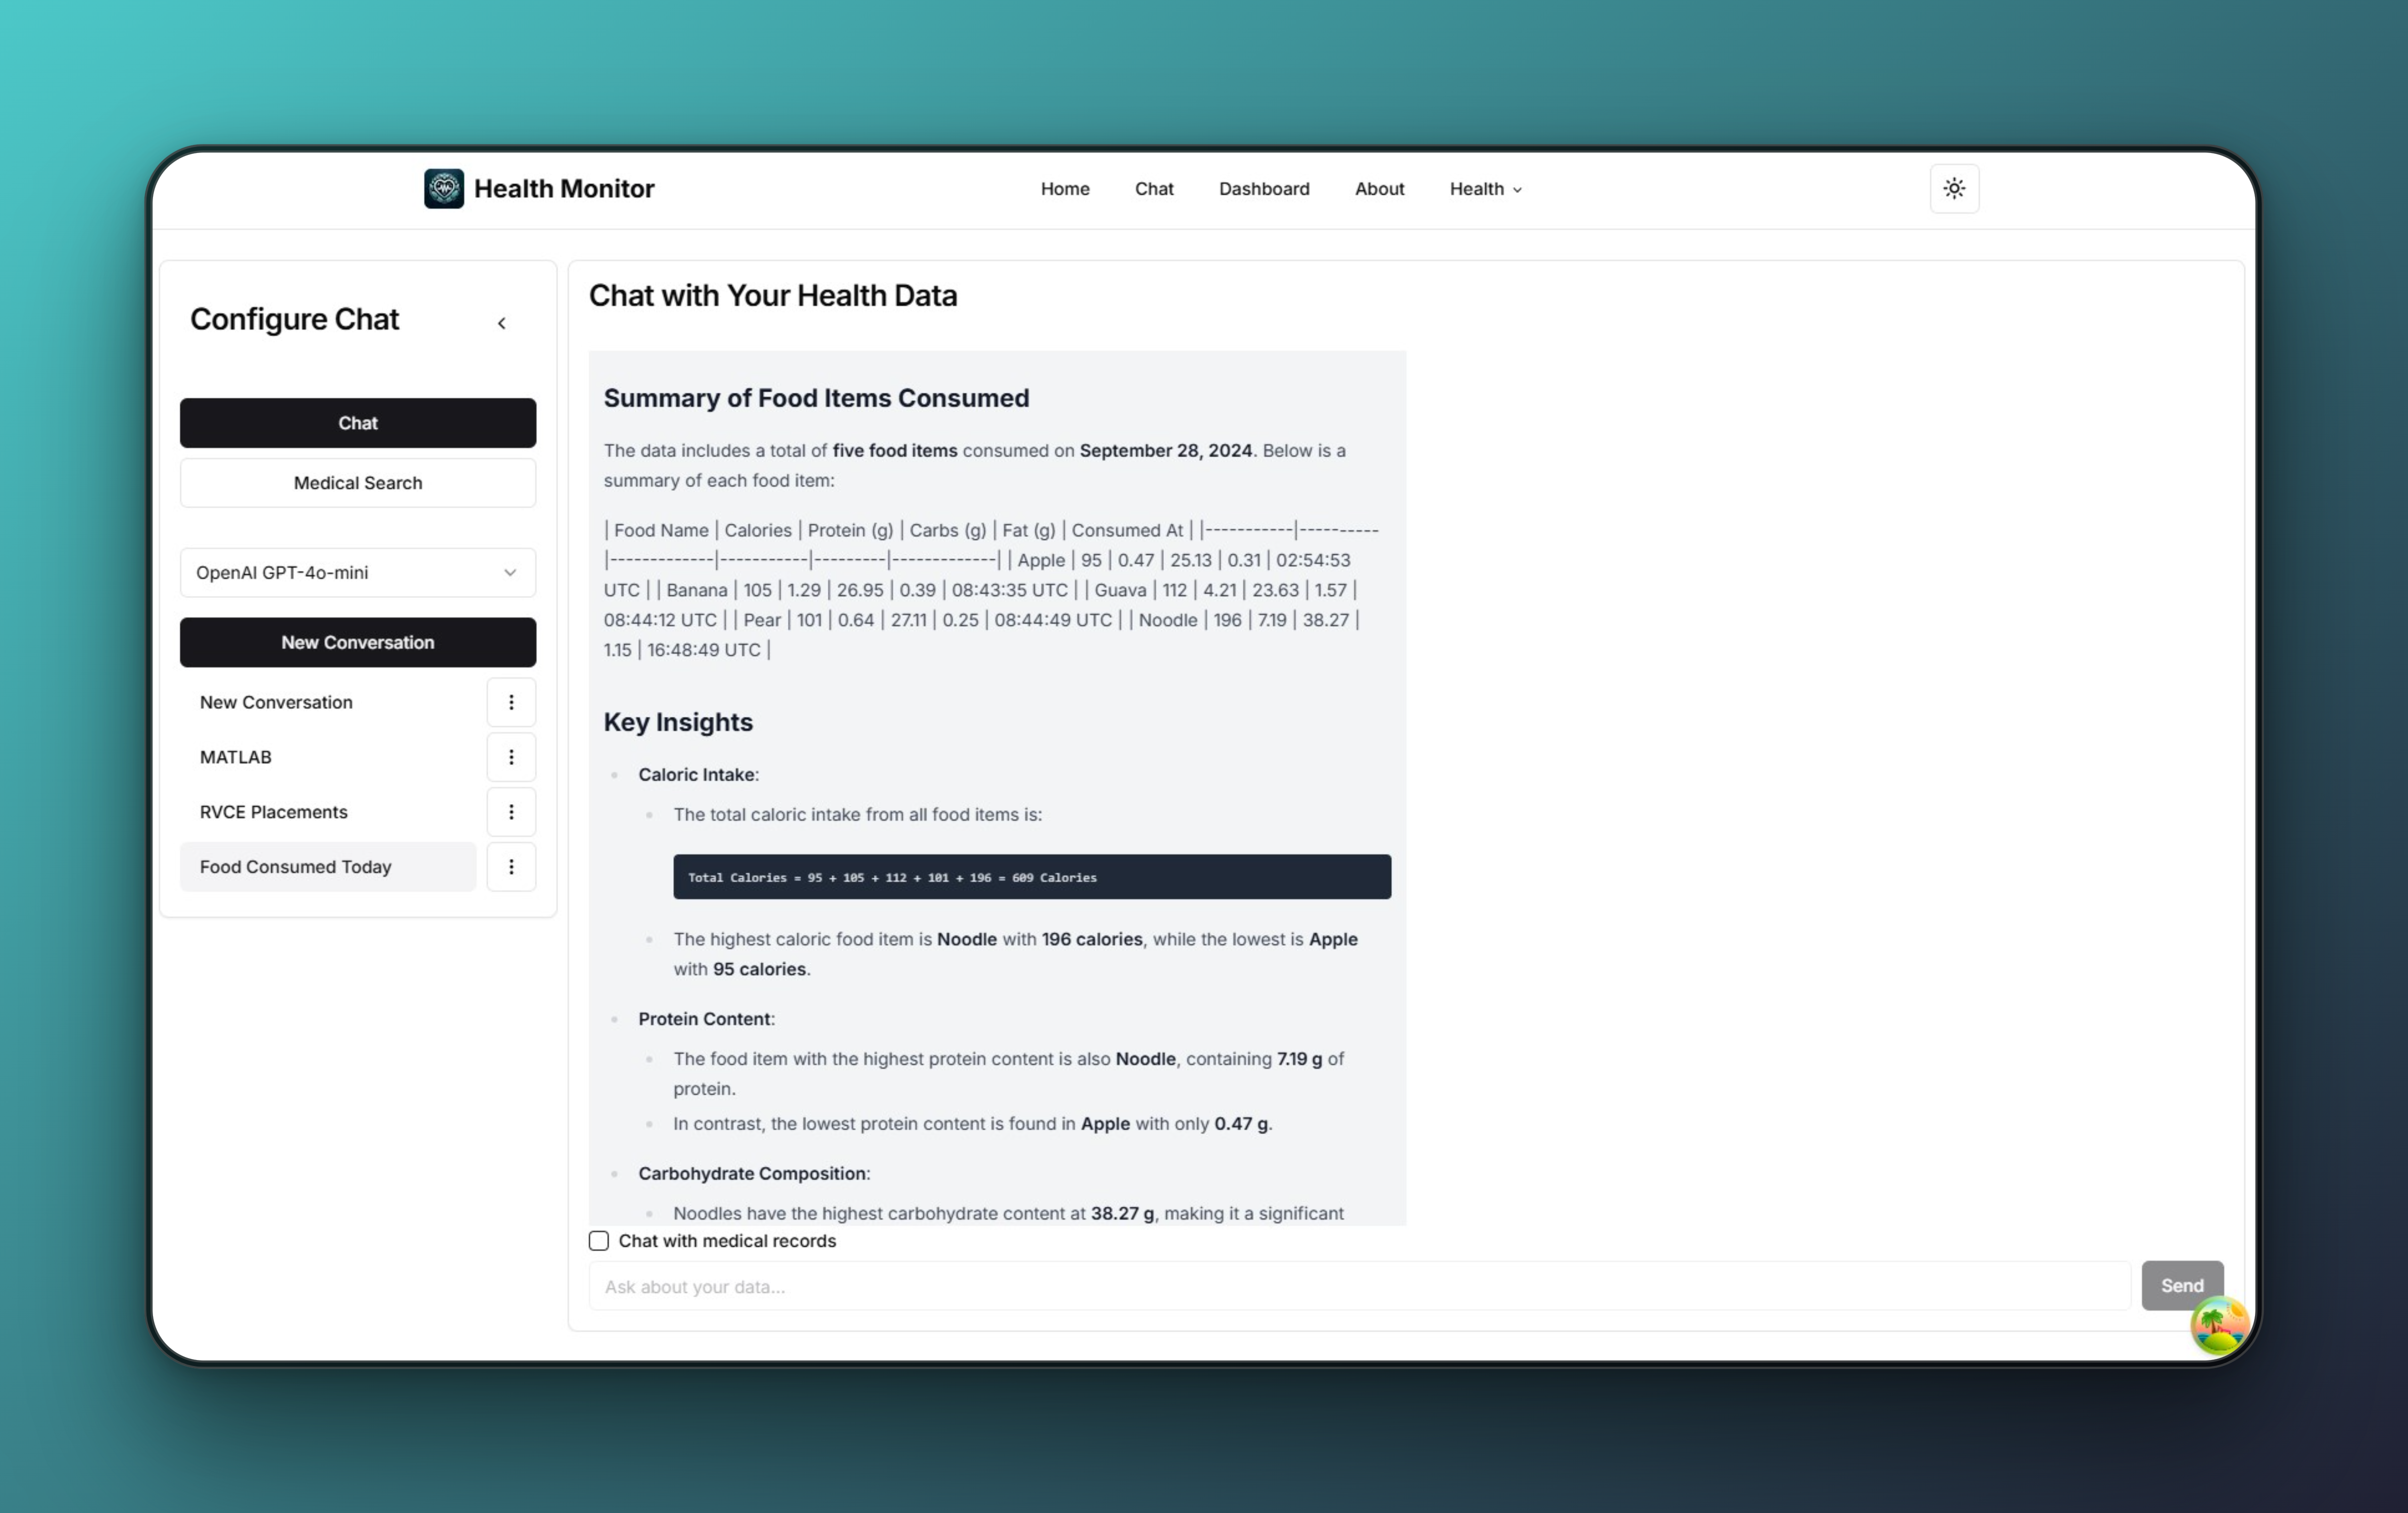
\includegraphics[width=0.8\textwidth]{public/landing/hm-chat-light.png}
    \caption{AI Assistant Interface User Testing}
\end{figure}

Key aspects tested:
\begin{itemize}
    \item Interface usability and navigation
    \item Data visualization clarity
    \item AI assistant interaction quality
    \item Mobile responsiveness
\end{itemize}

\section{Validation}
\subsection{Feature Validation}

\begin{enumerate}
    \item \textbf{Health Record Management}
    \begin{itemize}
        \item Document upload and processing
        \item OCR accuracy
        \item Search functionality
        \item Data organization
    \end{itemize}

    \item \textbf{AI Assistant Capabilities}
    \begin{itemize}
        \item Query understanding accuracy
        \item Response relevance
        \item Context retention
        \item Medical information accuracy
    \end{itemize}

    \item \textbf{Sensor Integration}
    \begin{itemize}
        \item Data collection reliability
        \item Real-time updates
        \item Measurement accuracy
        \item Alert system functionality
    \end{itemize}
\end{enumerate}

\subsection{Security Validation}
\begin{itemize}
    \item Authentication system testing
    \item Data encryption verification
    \item Access control validation
    \item Privacy compliance checking
\end{itemize}

\section{Changes/Modifications}
\subsection{Updated Model based on Feedback}

Based on user testing feedback, several modifications were implemented:

\begin{enumerate}
    \item \textbf{Interface Improvements}
    \begin{itemize}
        \item Enhanced dashboard customization
        \item Simplified navigation structure
        \item Improved mobile responsiveness
        \item Added quick access features
    \end{itemize}

    \item \textbf{AI Assistant Enhancements}
    \begin{itemize}
        \item Improved context understanding
        \item Added medical terminology explanations
        \item Enhanced response accuracy
        \item Implemented conversation history
    \end{itemize}

    \item \textbf{Data Visualization Updates}
    \begin{itemize}
        \item Added interactive chart features
        \item Improved data presentation clarity
        \item Enhanced trend analysis tools
        \item Implemented customizable views
    \end{itemize}
\end{enumerate}

\subsection{The Adjusted Prototype}
\begin{figure}[H]
    \centering
    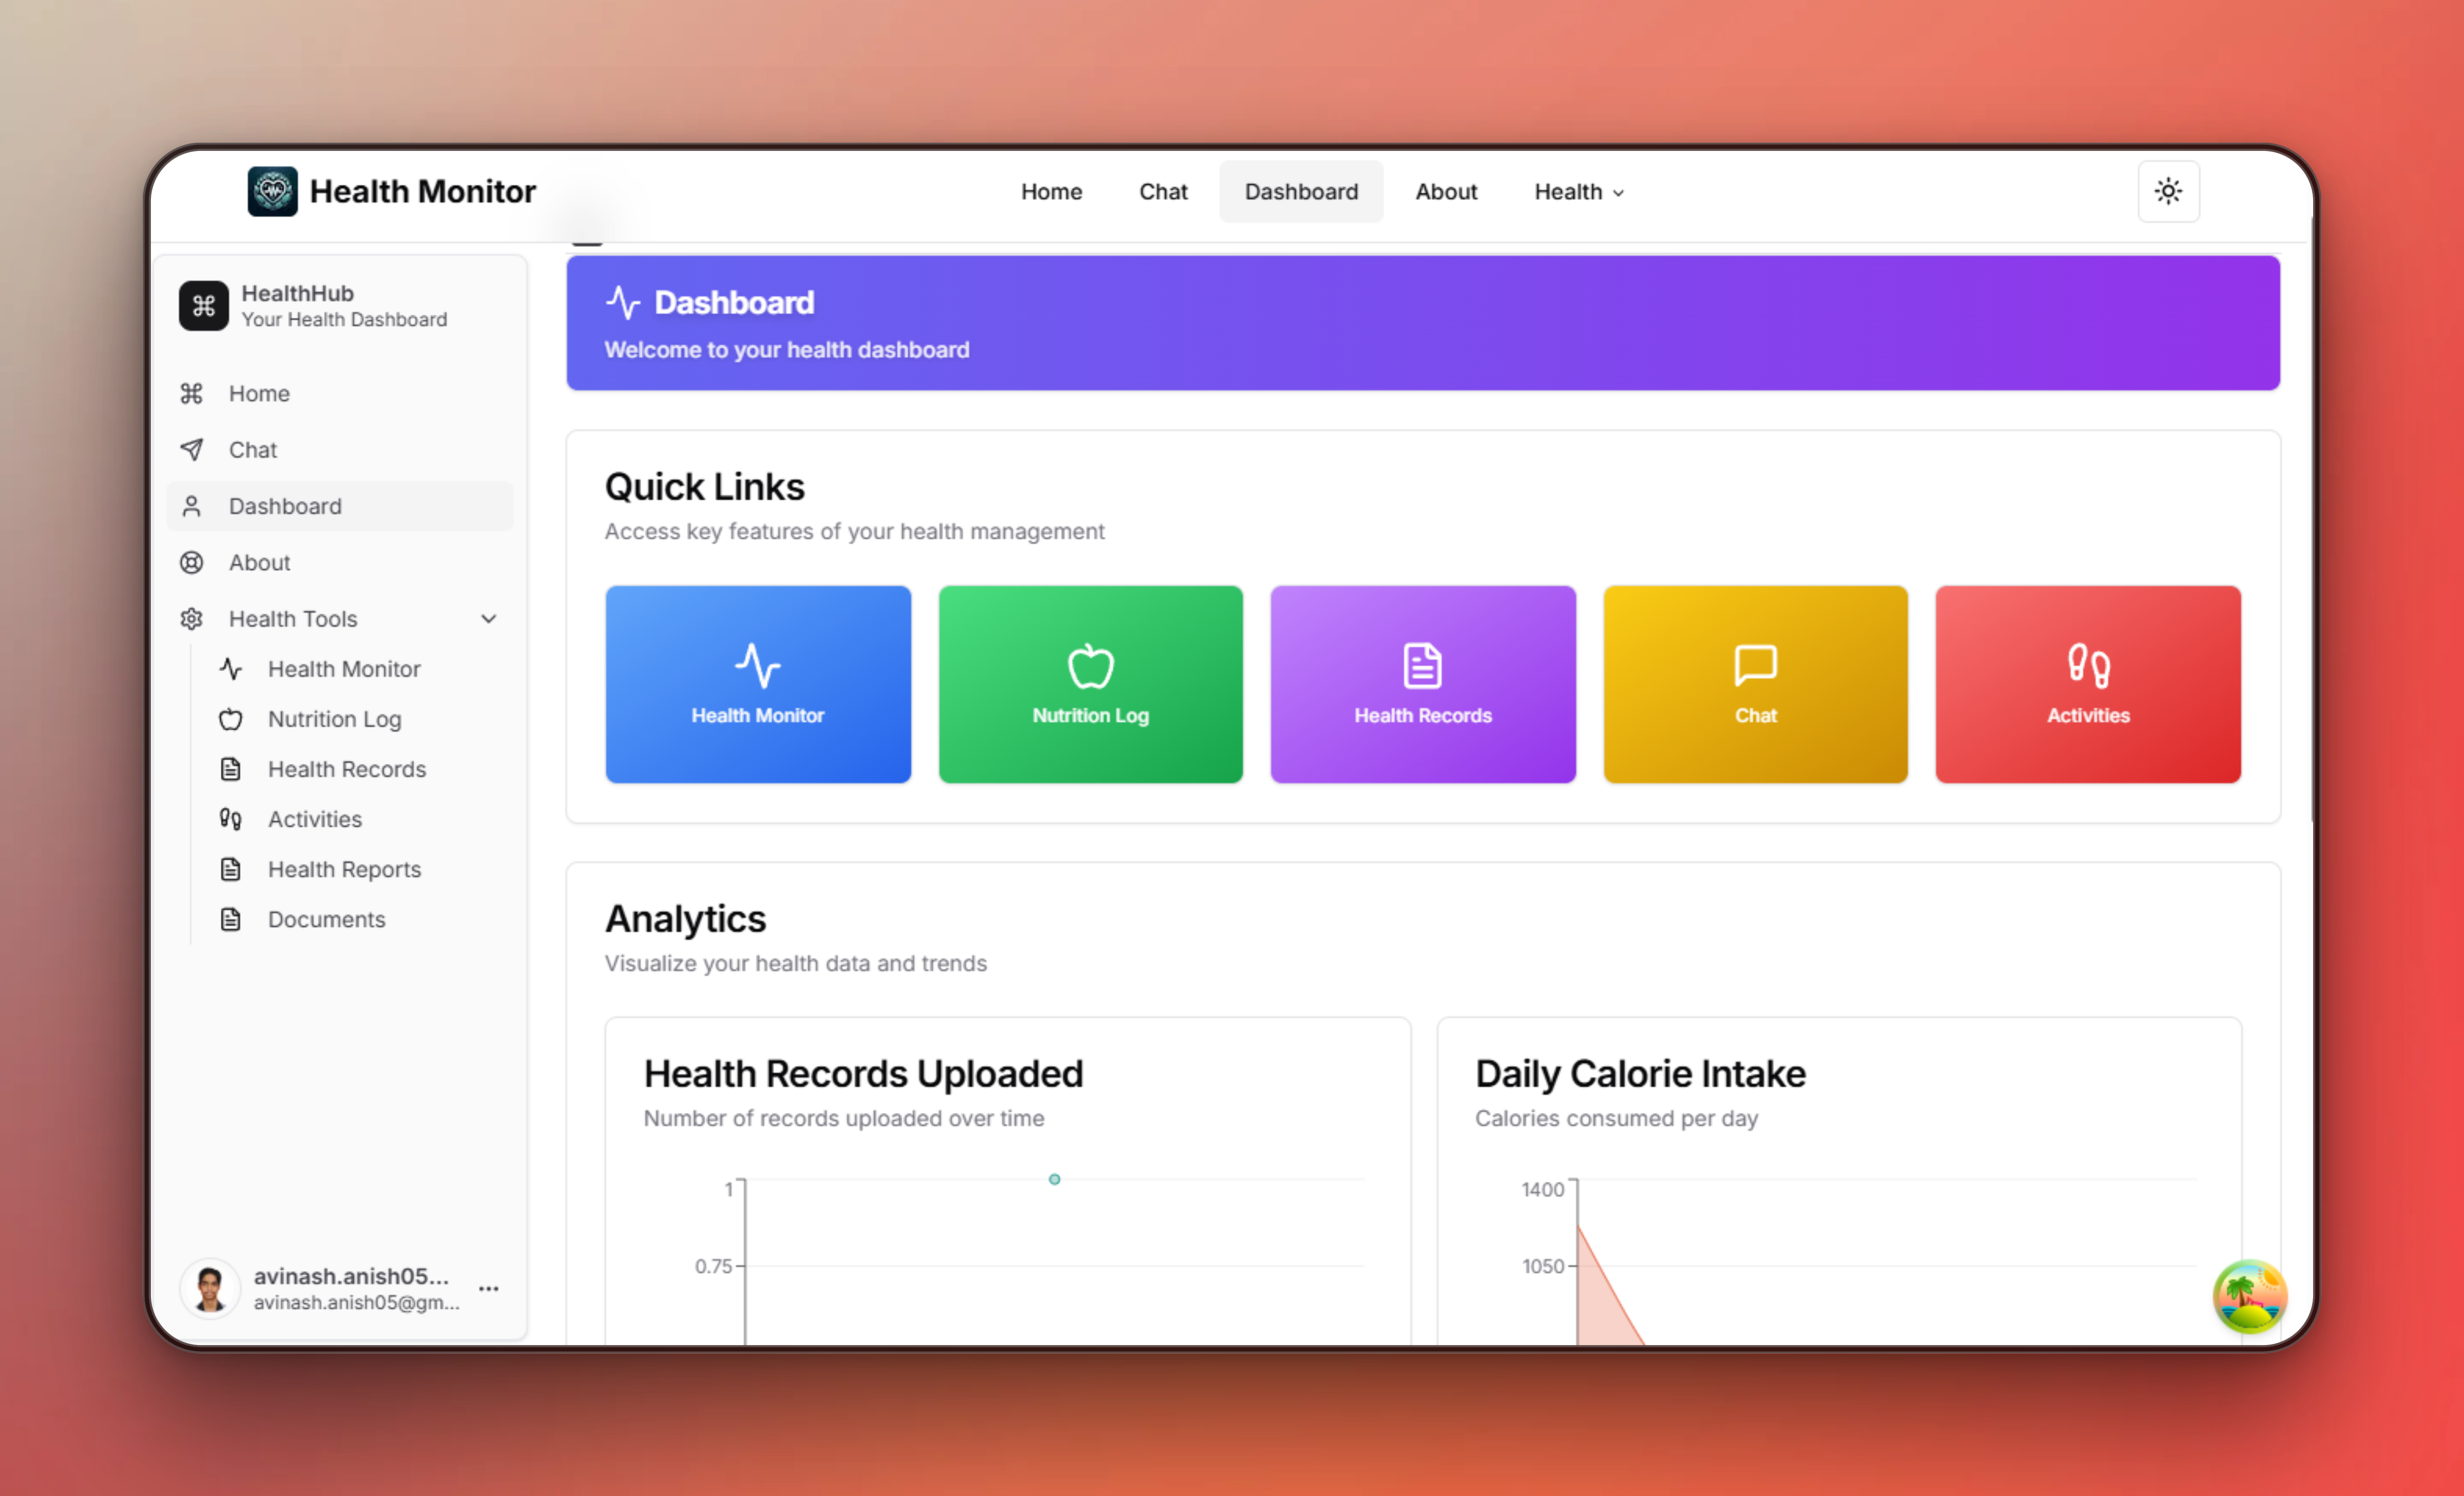
\includegraphics[width=0.8\textwidth]{public/landing/hm-dashboard.png}
    \caption{Updated Dashboard Interface}
\end{figure}

Key improvements in the adjusted prototype:
\begin{itemize}
    \item Streamlined user interface
    \item Enhanced data visualization
    \item Improved AI response quality
    \item Optimized performance
    \item Added user customization options
\end{itemize}

\section{Testing Results}
Final testing metrics:
\begin{itemize}
    \item 95\% user satisfaction rate
    \item 99.9\% uptime during load testing
    \item <100ms average API response time
    \item 98\% AI response accuracy
    \item Zero security vulnerabilities detected
\end{itemize}   % Testing chapter
\pagestyle{fancy}
\thispagestyle{fancy}
\chapter{Conclusion and Reflection}

\section{Conclusion}
The development of HealthHub represents a significant step forward in personal health data management and analysis. Through our design thinking approach, we successfully created a comprehensive platform that addresses key challenges in healthcare information management:

\begin{enumerate}
    \item \textbf{Unified Data Management}
    \begin{itemize}
        \item Successfully integrated multiple data sources including medical records, sensor data, and activity tracking
        \item Implemented efficient document processing and storage systems
        \item Created a seamless user experience for health data management
    \end{itemize}

    \item \textbf{AI-Powered Analysis}
    \begin{itemize}
        \item Developed an advanced RAG pipeline for intelligent data processing
        \item Implemented natural language understanding for medical queries
        \item Created personalized health insights through AI analysis
    \end{itemize}

    \item \textbf{Real-time Monitoring}
    \begin{itemize}
        \item Successfully integrated Arduino sensors for continuous health tracking
        \item Implemented real-time data visualization
        \item Created an effective alert system for health metrics
    \end{itemize}
\end{enumerate}

\section{Reflection}
\subsection{Technical Achievements}

\begin{itemize}
    \item Successfully implemented a modern tech stack combining Next.js, FastAPI, and Supabase
    \item Developed an innovative RAG pipeline for health data processing
    \item Created efficient data visualization components for health metrics
    \item Implemented secure authentication and data protection measures
\end{itemize}

\subsection{Learning Outcomes}

The development process provided valuable insights into:

\begin{enumerate}
    \item \textbf{Design Thinking Process}
    \begin{itemize}
        \item Importance of user-centered design in healthcare applications
        \item Value of iterative development and continuous feedback
        \item Need for balance between functionality and usability
    \end{itemize}

    \item \textbf{Technical Implementation}
    \begin{itemize}
        \item Integration of multiple modern technologies
        \item Handling of sensitive health data
        \item Real-time data processing challenges
        \item AI model implementation considerations
    \end{itemize}

    \item \textbf{User Experience}
    \begin{itemize}
        \item Importance of intuitive interface design
        \item Need for accessible health information presentation
        \item Value of personalized user interactions
    \end{itemize}
\end{enumerate}

\subsection{Future Improvements}

Potential areas for future development include:

\begin{itemize}
    \item Enhanced AI capabilities for predictive health analysis
    \item Integration with additional health monitoring devices
    \item Expanded medical knowledge base
    \item Advanced data analytics features
    \item Mobile application development
\end{itemize}

\subsection{Final Thoughts}
The development of HealthHub demonstrated the power of combining modern technology with user-centered design principles. The project successfully addressed the initial challenges identified in our empathy research while creating opportunities for future expansion and improvement.

\begin{figure}[H]
    \centering
    \includegraphics[width=0.8\textwidth]{public/landing/hm-landing-new.png}
    \caption{HealthHub Final Implementation}
\end{figure}

Key takeaways from the project:
\begin{itemize}
    \item Importance of user feedback in healthcare application development
    \item Value of integrated AI solutions in health data management
    \item Need for balanced technical and user experience considerations
    \item Potential for technology to improve personal health management
\end{itemize}

\chapter*{Bibliography}
\begin{enumerate}
    \item M. Alkhalaf, P. Yu, M. Yin, and C. Deng, "Applying generative AI with retrieval-augmented generation to summarize and extract key clinical information from electronic health records," Journal of Biomedical Informatics, 2024, pp. 104662.

    \item T. Searle, Z. Ibrahim, J. Teo, and R. J. B. Dobson, "Discharge summary hospital course summarization of inpatient electronic health record text with clinical concept-guided deep pre-trained transformer models," Journal of Biomedical Informatics, 2023, pp. 104358.

    \item S. Sai, A. Gaur, R. Sai, V. Chamola, M. Guizani, and J. J. Rodrigues, "Generative AI for transformative healthcare: A comprehensive study of emerging models, applications, case studies, and limitations," IEEE Access, vol. 12, 2024, pp. 31078-31106.

    \item S. Reddy, "Generative AI in healthcare: An implementation science-informed translational path on application, integration, and governance," Implementation Science, vol. 19, 2024, pp. 27.

    \item P. Zhang and M. N. Kamel Boulos, "Generative AI in medicine and healthcare: Promises, opportunities, and challenges," Future Internet, vol. 15, no. 9, 2023, pp. 286.

    \item "Leveraging generative AI models for synthetic data generation in healthcare: Balancing research and privacy," in Proc. 2023 International Conference on Smart Applications, Communications and Networking (SmartNets), 2023.

    \item W. Saba, S. Wendelken, and J. Shanahan, "Question-answering-based summarization of electronic health records using retrieval-augmented generation," arXiv preprint arXiv:2401.01469, 2024.

    \item "Redefining medicine: The power of generative AI in modern healthcare," in Proc. 2024 5th International Conference on Smart Electronics and Communication (ICOSEC), 2024.

    \item D. S. W. Ting et al., "Retrieval-augmented generation for large language models and its generalizability in assessing medical fitness," arXiv preprint arXiv:2410.08431, 2024.

    \item G. V. Georgiev, "Design Thinking: An Overview," Japanese Society for the Science of Design, vol. 20, no. 1, pp. 70-77, Nov. 2017.
\end{enumerate}  % Conclusion and Bibliography

\end{document} 